
In this chapter we will dive into how FluiDB processes and handles
queries up to logical planning. Query processing is at the heart of
FluiDB. We will start by looking into see what kinds of queries FluiDB
can read and how it reads them. Then we will look at how it relates
the queries with each other to construct a tightly interrelated story
of the workflow by looking at the basic query graph, the heart of
FluiDB. Then we will look at some initial query processing that FluiDB
depends on to extract information from individual queries. Then we
will look at how FluiDB normalizes queries in order to determine when
queries are equivalent and when they are not. Then we will look at how
clusters representing single operations are formed within the query
graph and how those are used to keep in sync information about
intermediate results. Finally, we conclude by descibing how the query
processing infrastructure, which sits at the core of the RDBMS,
interfaces with the rest of the components: the planner, Antisthenis
and the code generator, described in later chapters.

\section{System overview and the query graph}
\label{sec:optimizer_system_overview}
With the advent of technologies that make access to information
scalable and affordable, the mental and temporal gap between
collection of data and their analysis grows rapidly. At least two of
the biggest players in the the tech industry, Facebook and Google,
base their competitive advantage on vast amounts of information that
they have collected and their capacity for such collection. In cases
like these the layout of the stored data is independent of the growing
number of applications taking advantage of it. We believe there are
opportunities in automatically and dynamically optimizing data
representation to fit the workload.

Consider for example the following query over the TPC-H dataset that
computes the average discount per country:

\begin{listing}[p]
  \begin{minted}[]{sql}
    select      n_name, avg(l_discount)
    from        lineitem, customer, nation, order
    where       l_orderkey = o_orderkey
    and         c_custkey = o_custkey
    and         c_nationkey = n_nationkey
    and         l_shipdate > 10-11-2015
    group by    n_name
  \end{minted}
  \caption{The sql query}
\end{listing}

An optimizer considering this query in isolation might come up with
the following plan following plan:

\begin{figure}[p]
  \centering
  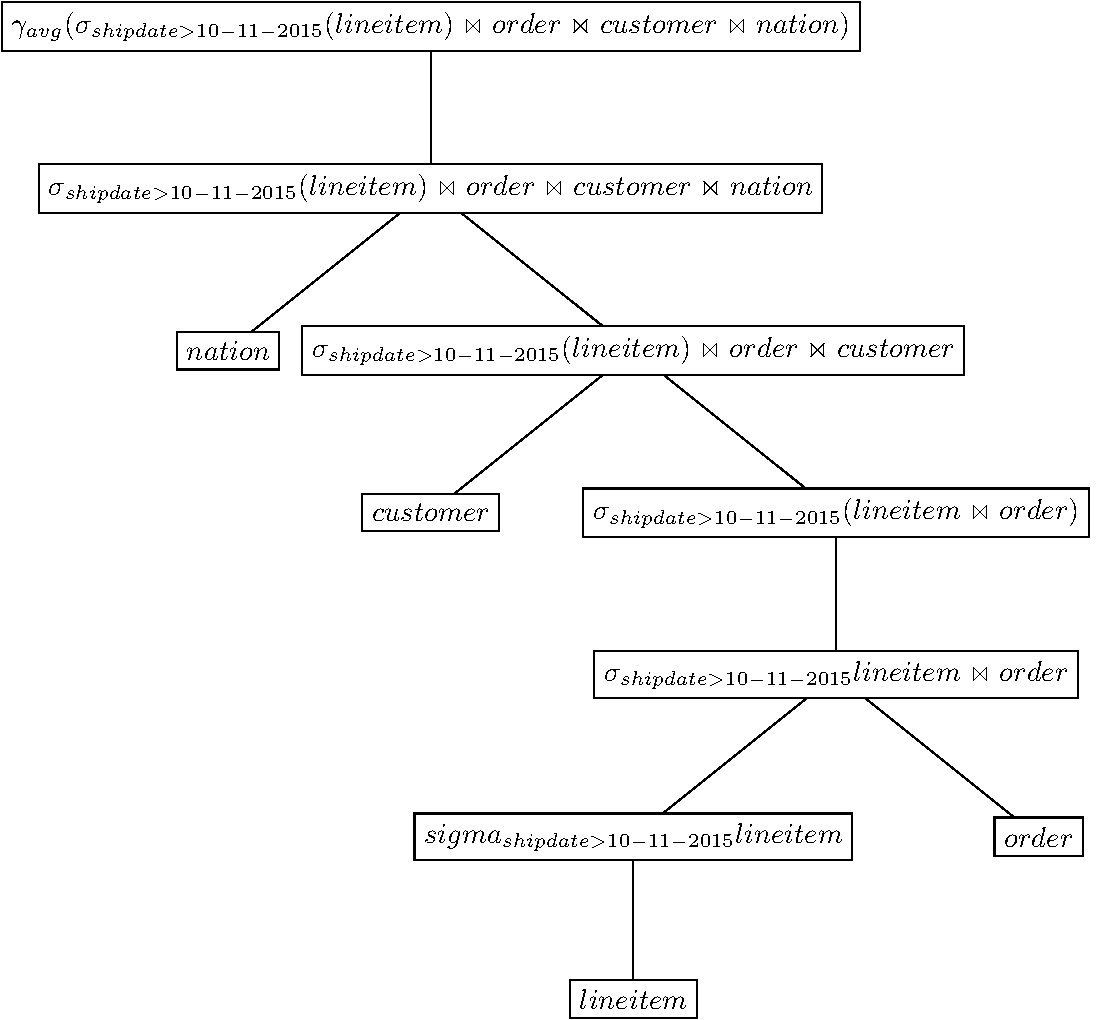
\includegraphics[width=.9\linewidth]{./imgs/optplan.pdf}
  \caption{\label{fig:optplan}A possible optimal plan for an isolated query.}
\end{figure}

However, for certain workloads it might be more beneficial to opt for
a plan that materializes the relation \(lineitem \Join order\) and the
relation \(customer \Join nation\) so they can be used to optimize
later queries. In that case, even if the most beneficial plan for the
isolated query is deemed to be the one shown in figure \ref{fig:optplan},
taking a holistic view of a workload during query planning making
heavy use of \(lineitem \Join order\) and \(customer \Join nation\) a
better choice would be what appears in figure \ref{fig:workplan}.

\begin{figure}[p]
  \centering
  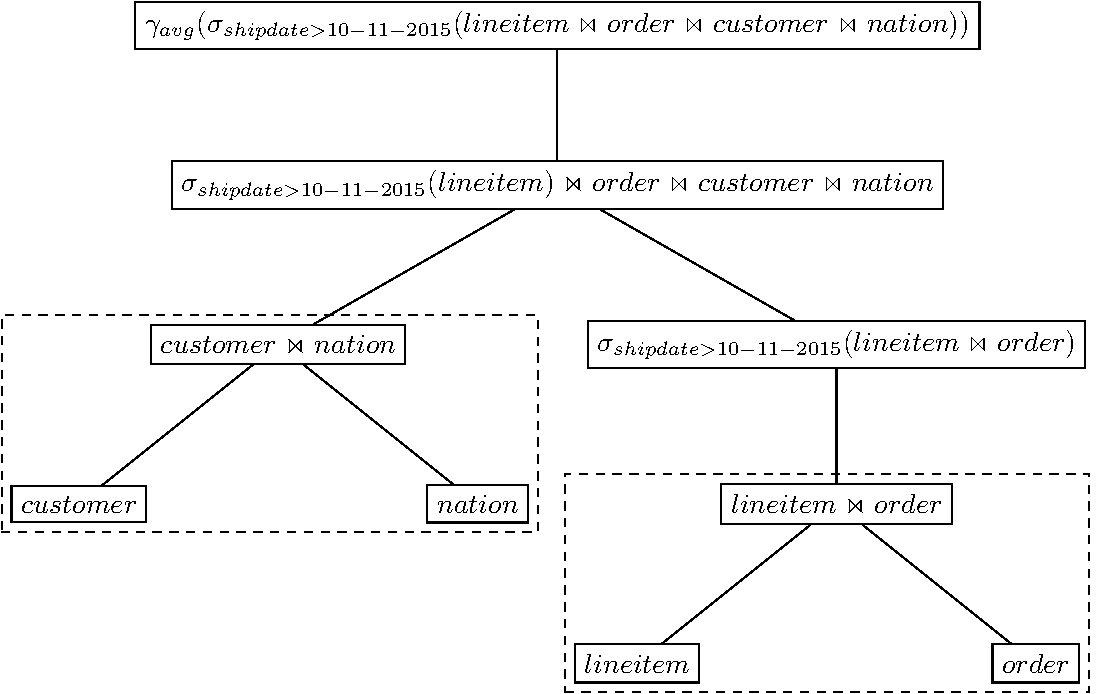
\includegraphics[width=.9\linewidth]{./imgs/workplan.pdf}
  \caption{\label{fig:workplan}A possible optimal plan for a sequence of queries that makes heavy use of \(lineitem \Join order\) and \(customer \Join nation\)}
\end{figure}

A simple but effective solution to addressing the problem of
integrating incremental query materialization and the optimization
processes, was presented in
\cite{perezHistoryawareQueryOptimization}. In their approach they
maintain a \emph{history pool} (a list of all the past queries) that is
used to decide the benefit of materializing a sub-expression, and a
\emph{view pool} that keeps track of the materialized tables at every
moment. Both these sets are taken into account during planning to
produce a plan that will likely minimize the amortized cost of the
workload. After the query is solved the sets are updated. A limitation
of such an approach is that when dealing with relations like
\(lineitem \Join order\) in budget restricted settings, materialized
view storage can quickly become a scarce resource.

There is an opportunity to reduce the effect of this problem by
exploiting another common workload attribute: certain tables are
frequently subsumed by the same intermediate result. In the case of
our example it may be the case that, within our hypothetical workload,
whenever the \(lineitem\) or the \(order\) tables are encountered in a
query, they can usually be subsumed by the \(lineitem \Join order\)
relation. In other words, when both \(lineitem \Join order\) and
\(lineitem\) (or \(order\)) are materialized it is preferable to only use
\(lineitem \Join order\) in the query plan. Since most of the data of
\(lineitem\) and \(order\) are also in \(lineitem \Join order\), it might
make sense, instead of maintaining the \(lineitem\) and \(order\) tables
separately, to keep \(lineitem \Join order\) and enough information to
reconstruct \(lineitem\) or \(order\) when needed.

We propose a solution to both those problems resembles the solution
provided in \cite{gouSupSearchEfficient2006} by Gou et.al. In their work
they embed aggregations \texttt{group by x1, .., xk} into the
\(\subseteq\)-lattice that arises from the powerset \(P(\{x_1, ...,
x_k\})\). Thereby they encode the fact that \texttt{group by A, B, C} is
subsumed, or can be computed by, either of \texttt{group by A, B}, \texttt{group by
  A, C} or \texttt{group by B, C}. Once the lattice is constructed a variant of
the \(A^{\star}\) path finding is used algorithm to search for the
optimal aggregation plan. However \cite{gouSupSearchEfficient2006} on
the one hand makes no attempt to recycle tables, ie. garbage collect
tables, whose data can be found in other relations, and narrows it's
attention to aggregations.

From the aforementioned work we keep the basic notion of using a graph
to represent the subsumption of queries and to derive the benefit of
materializing a relation. We also use path finding techniques in that
graph to create plans. However we introduce a more complex and ad-hoc
hierarchy of relations to account for subsumptions the entire
relational algebra, rather than just aggregations that is very similar
to AND-OR dags as found in
\cite{mistryMaterializedViewSelection2001}. Thereby we express for
example the fact that \(\sigma_p(S)\) subsumes \(\sigma_{p \lor q}(S)\),
or that \(B \Join C\) subsumes \(A \Join B \Join C\). Furthermore the
relations we express in that graph are bidirectional. So rather than
only finding paths towards the goal and deleting relations when they
are no longer needed, we simultaneously plan for moving towards the
goal query and performing "backwards" operations for saving up
space. We clarify this with an example which demonstrates a slightly
simplified version of our system's functionality.

In figure \ref{fig:intro_selectexample} we provide representation of a subsumption
graph that our RDBMS might create after witnessing selections on
\(lineitem\). For brevity let \(p:=shipdate > 10-11-2015\),
\(q:=quantity < 24\) and \(r:=discount < .06\). The RDBMS has
encountered \(\sigma_{p}(lineitem)\), \(\sigma_{q}(lineitem)\) and
\(\sigma_{q} \sigma_{r} (lineitem)\).

\begin{figure}[p]
  \centering
  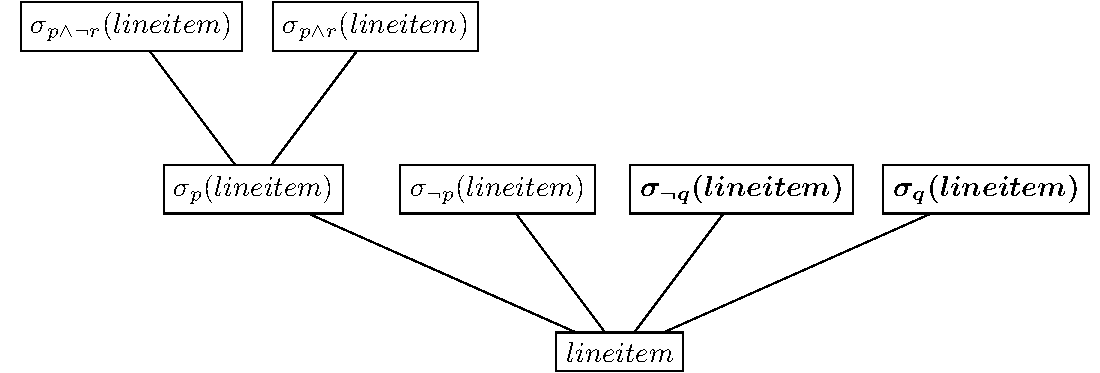
\includegraphics[width=.9\linewidth]{./imgs/intro_selectexample.pdf}
  \caption{\label{fig:intro_selectexample}Any relation can be selected in different ways forming a tree can be further split on top of that.}
\end{figure}

With \(\boldsymbol{bold}\) we mark the materialized relations. The query
that we are solving is \(\sigma_{quantity < 24} \sigma_{discount < .06}
(lineitem)\), which is denoted in the figure as \(\sigma_{q \land
  r}(lineitem)\). Our total size budget is 2.5.

Following the edges in the graph, to solve \(\sigma_{q \land
  r}(lineitem)\) we need \(\sigma_{q}(lineitem)\) and for that we need
\(lineitem\). So first the union:

\[
  \sigma_{\neg p}(lineitem) \cup \sigma_{p}(lineitem) \rightarrow lineitem
\]

Then we need \(\sigma_{q}(lineitem)\) but we are now using 2 units of
space and adding .6 more would exceed our space budget of
2.5. \(lineitem\) is the least beneficial of our materialized views
but it is required for our next step, ie. creating
\(\sigma_{q}(lineitem)\) . \(\sigma_{\neg p}(lineitem)\) is deleted
since it's derivable from \(lineitem\) and is least beneficial. Then
\(\sigma_{q}(lineitem)\) is created and now we are using 2.1 units of
space.

\[
  lineitem \rightarrow \sigma_{q}(lineitem)
\]

Finally we need to create the final relation \(\sigma_{q \land
  r}(lineitem)\) . However it's space requirement is .5 and we we would
be exceeding our budget. We can't delete \(lineitem\) even though it
is our least beneficial table because we would have no way of
recreating it.

Here we have two options. One is to delete \(\sigma_{\neg
  p}(lineitem)\), our most benefit al table. The other, which is the one
that the system should opt for, is to backtrack. When we created
\(\sigma_{q}(lineitem)\), instead we create both
\(\sigma_{q}(lineitem)\) and \(\sigma_{\neg q}(lineitem)\).

\[
  lineitem \rightarrow \{\sigma_{q}(lineitem), \sigma_{\neg q}(lineitem)\}
\]

Once both those tables are materialized we can safely delete
\(lineitem\). Now our space usage is 1.1 and we can safely

\[
  \sigma_{q}(lineitem) \rightarrow \sigma_{q \land r} (lineitem)
\]

Which is the requested query and, in summary, the final plan is:

\begin{align*}
  &\sigma_{\neg p}(lineitem) \cup \sigma_{p}(lineitem) \rightarrow lineitem \\
  &Delete[\sigma_{\neg p}(lineitem)] \\
  &lineitem \rightarrow \{\sigma_{q}(lineitem), \sigma_{\neg q}(lineitem)\} \\
  &Delete[lineitem] \\
  &\sigma_{q}(lineitem) \rightarrow \sigma_{q \land r} (lineitem)
\end{align*}

The key idea behind this work, which was demonstrated in the example,
is that a) by using reversible operations between relations and b) by
integrating the query planner and the materialized view recycling
mechanism, we get grater flexibility to adapt the data layout to the workload thereby
optimizing the use of our space budget.


\subsection{Relational Algebra semantics}
\label{sec:relational_algebra_semantics}
Much like most other RDBMSs, FluiDB deals with queries expressed in
therms of a \textbf{relational algebra}.  Here we define the relational
algebra semantics that is the traditional relational algebra extended
by unary operators for ordering \(s_e(X)\), limiting \(l_i(X)\) and
aggregating \(\gamma_e(X)\). Figure \ref{tab:org602cd71} lists list correspondences
between our relational algebra notation and the corresponding SQL.

\begin{table}[p]
  \caption{\label{tab:org602cd71}Correspondence between relational algebra expressions and SQL.}
  \centering
  \begin{tabular}{lll}
    Description & RA & SQL\\
    \hline
    Aggregation & \(\gamma_e(X)\) & \texttt{select * from X group by e}\\
    Ordering & \(s_e(X)\) & \texttt{select * from X order by e}\\
    Aggregation & \(l_i(X)\) & \texttt{select * from X limit i}\\
    Join & \(X \Join_p Y\) & \texttt{select * from X, Y where p}\\
    Anti-semijoin & \(X \lnsemi_p Y\) & \\
    Union & \(X \cup Y\) & \\
    Selection & \(\sigma_p(X)\) & \texttt{select * from X where p}\\
    Projection & \(\pi_r(X)\) & \texttt{select r from X}\\
  \end{tabular}
\end{table}

Before going any furhter it is important to clarify some assumptions
that FluiDB makes to operate. Particularly that \(\forall A,p
. \sigma_p A \cup \sigma_{\neg p} A \equiv A\). This means that there
no \texttt{NULL} values are allowed since a predicate over a NULL value
always evaluates to \texttt{False}. Further we assume set semantics for all
relations. Any valid expression needs to have at least one unique
subtuple. The user is not burdained with the responsibility of
enforcing this, but rather pre-process projections and aggregations on
any query immediately after it is being parsed so that unique columns
of the primary are exposed (see section on \hyperref[sec:orgd903905]{query preprocessing}).

The sematics of the sorting operation are preserved by making a small
concession to the set semantics: The \emph{only} time when records of a
relation are assumed to be ordered is for expressions of the form
\(s_e(X)\) and only for the duration between it running and the next
operation.

With those out of the way we can talk about the antijoin operator
\(\lnsemi_p\) . It is equivalent to \(A \lnsemi_p B \equiv A \backslash
\pi_A(A \Join_p B)\) and it is primarily useful for creating a
bidirectional join by capturing the rows left over from a join (see
subsection on the \hyperref[sec:org5a9ec3b]{QDAG}). The important property we will be interested
in is:

\[
  A \lnsemi_p B \cup \bar\pi_A(A \Join_p B) \equiv A
\]

\(\bar{\pi}_{cols(A)}\) means group by the unique columns of \(A\).  As
syntactic sugar we also define:

\[
  A \rnsemi_p B := A \lnsemi_{\neg p} B
\]

It is important to be noted that the semantics assumed by for the RA
consider relations with different order of columns to be semantically
equivalent in all situations.

\subsubsection{Expressions}
\label{sec:orgaa9cf48}

Relational algebra expressions contain expressions that operate at the
field level. These are in projection column definitions, selection
predicates, aggregation column definitions, etc. These lower level are
organized in up to 4 distinct layers based on the kinds of operators
in order to make it easier to type functions that operate on only some
of the layers:

\begin{itemize}
\item The top layer is purely boolean operations \texttt{Prop}. This layer can
  thake the CNF form as an AND of ORs. The type of the layer is
  presented in listing \ref{org9949756}. This layer is nested.
\item The intermediate layer \texttt{Rel} describes relations between values
  (\(\equiv\), \texttt{like}, \(<\), \(\le\), etc). This layer is not
  nested, ie we do allow define relations between relations
  \ref{orge4b33ce}.
\item The lowest layer \texttt{Expr} is expressions of any kind that may return
  any value. The above layers can be expressed in terms of this layer
  because in order to support the ternary operator \texttt{if <expr> then
    <expr> else <expr>}. Its definition can be foun in listing \ref{org66d9c80}.
\item The symbol layer that in most parts of FluiDB leave the symbol
  type. This allows us to tag the symbols in the expression without
  breaking compatibility.
\end{itemize}

Predicates of selections and joins (joins are always \(\theta\) joins
at the type level) have type \texttt{Prop (Rel (Expr e))} for some type \texttt{e}
and projections have type \texttt{QProj [(e,Expr e)]}. A special layer is
provided for aggregations \texttt{Aggr} see \ref{org9a5f75b} that makes it
possible to disallow nested aggregation functions at the type level
making the aggregation operator \texttt{QGroup [(e,Expr (Aggr (Expr e)))]
  [Expr e]}, where the first argument of the constructor is the
aggregation functions and their names, and the sectond argument is the
expressions on which the grouping should happen.

Further inverui

\begin{listing}[p]
  \begin{haskell}
    data Prop a = P2 BPOp (Prop a) (Prop a)
      | P1 UPOp (Prop a)
      | P0 a
    data UPOp = PNot
    data BPOp = PAnd | POr
  \end{haskell}
  \caption{\label{org9949756}Definition of a proposition, a boolean expression}
\end{listing}

\begin{listing}[p]
  \begin{haskell}
    data Expr s = E2 BEOp (Expr s) (Expr s)
      | E1 UEOp (Expr s)
      | E0 s
    data UEOp =
      EFun ElemFunction
      | ENot
      | EAbs
      | ESig
      | ENeg
    data ElemFunction
      = ExtractDay -- erased after parsing
      | ExtractMonth -- erased after parsing
      | ExtractYear -- erased after parsing
      | Prefix Int
      | Suffix Int
      | SubSeq Int Int
      | AssertLength Int
    data BEOp =
      -- Boolean (truthy)
      EEq
      | ELike
      | EAnd
      | EOr
      | ENEq
      -- Numeric
      | EAdd
      | ESub
      | EMul
      | EDiv
  \end{haskell}
  \caption{\label{org66d9c80}Definition of an expression.}
\end{listing}

\begin{listing}[p]
  \begin{haskell}
    data Rel a = R2 BROp a a
    data BROp
      = REq
      | RGt
      | RLt
      | RGe
      | RLe
      | RLike
      | RSubstring
  \end{haskell}
  \caption{\label{orge4b33ce}Definition of a relation expression expression}
\end{listing}

\begin{listing}[p]
  \begin{haskell}
    data AggrFunction = AggrSum
      | AggrCount
      | AggrAvg
      | AggrMin
      | AggrMax
      | AggrFirst
    \end{haskell}
  \caption{\label{org9a5f75b}Definition of an aggregation expression}
\end{listing}


\subsection{QDAG: The unified query graph}
\label{sec:org5a9ec3b}
The operation of FluiDB revolves around an AND-OR graph of relations
and algebraic operations. not unlike ones used in the multiquery
optimizations. This graph encodes all the plans that the query
optimizer and planner will consider by means of traversal. It will
become clear what that means in a moment. Said graph is a bipartite
graph where t-nodes (AND nodes in other literature) represent
relational operations and n-nodes (OR nodes elsewhere) represent
relations that will act as intermediate results. Before we consider
our introduced extensions we describe the basic operation of the
graph:

\begin{itemize}
\item There are multiple ways of composing relational operations to
  materialize a certain relation. Each one is a relational algebraic
  representation and we commonly refer to them as logical plans. Each
  one are represets trees similar to an abstract syntax tree. These
  trees are made of two kinds of nodes: operation nodes, t-nodes, and
  relation nodes, n-nodes. For example the query \(A \Join B \Join C\)
  may be represented as \((A \Join B) \Join C\) or
  \(A \Join (B \Join C)\) due to associativity of \(\Join\). Those two
  represent two tree forms where the join operators \(\Join\) are
  represented as t-nodes and each of \(A\), \(B\), \(C\),
  \(A \Join B\), \(B \Join C\) and \(A \Join B \Join C\) are
  represented as n-nodes.
\item All possible logical plans of a query are enumerated. The DAG of
  a query is created by unifying all these logical plans by means of
  merging n-nodes that are equivalent. For example the mentioned trees
  \((A \Join B) \Join C\) and \(A \Join (B \Join C)\) shared the nodes
  \(A \Join B \Join C\), \(A\), \(B\) and \(C\).
\item Each n-node can be materialized by triggering one of the input
  t-nodes. In other words by running a connected operation to which
  said n-node is on the output. It is clear then where the name
  OR-node found in other literature originates: any of the input nodes
  may participate to a plan involving the OR-node (n-node for
  us). Conversely each t-node can be triggered iff all of it's input
  n-nodes are materialized. Because \emph{all} input nodes must be
  materialized, t-nodes are elsewhere refered to as AND-nodes.
\item A global DAG is maintained into which the constructed DAGs of
  all consdered queries are merged, again, by merging equivalent
  n-nodes, where equivalent n-nodes are ones that refer to equivalent
  relations.
\item From a DAG we can derive logical plans for queries. We shall refer
  to the encapsulating this functionality as the \emph{planner}. The
  planner operates in terms of this global DAG. It traverses the DAG
  searching for a plan (ie a sequence of t-node triggers) that will
  cheaply materialize the requested node(s). This way nodes are
  naturally considered. The problem of reusing materialized
  intermediate results is thereby conceptualized as a graph traversal
  problem.
\item During this planning process, if storage space runs out, the
  garbage collector (GC) is triggered. Garbage collection in this
  context is the process of deleting materialized relations that are
  not used for the query at hand. We shall say that an n-node is
  \emph{deleted} when the garbage collector appends to the plan a delete
  operation that removes the corresponding materialized relation
  from storage.
\end{itemize}

In our particular case queries are solved one at a time. Each query is
transformed into a DAG and inserted in the graph. Then the root node,
that represents the solution to the query, is solved. This technique
borrowed by the field of multiquery optimization (MQO) helps us with
integrating the consideration of historical queries into the
optimization process. In contrast multiquery optimization algorithms
like \cite{mistryMaterializedViewSelection2001} we solve a different
problem: rather than optimizing a batch of queries, we try to plan for
each query in a sequence of them, optimizing for the amortized cost
under storage budget constraints.

We modify this conception of the DAG in a simple yet important way:
each t-node may have multiple outputs and can be partially
bidirectional. In other words a t-node, as well as multiple inputs,
may have multiple outputs, any number of which may be materialized by
it being triggered. A \emph{reverse trigger} of said t-node would
materialize inputs provided that all outputs are materialized and
under certain other conditions on which we will elaborate shortly. In
other words, where AND-nodes are similar to functions that when
evaluated produce an output given some input, t-nodes correspond to
bidirectional relations between sets of input and output
relations. This not only creates opportunities in terms of what plans
are possible, but also opens the gate to a whole new regime for how
garbage collection is involved in the process of query planning. Any
n-node may potentially be garbage collected, even primary tables, as
long as the garbage collector can prove that it is reconstructable by
triggering or reverse triggering t-nodes. The storage budget is
thereby taken into account not only when selecting or rejecting
materialized views, but also while planning the query solution
itself. We shall refer to the DAG we just described as simply DAG
where it is clear from context or tn-DAG when it is contrasted with
the AND-OR DAG.

To make this process clearer, as an example, consider a DAG that
contains just a selection:

\begin{figure}[p]
  \centering
  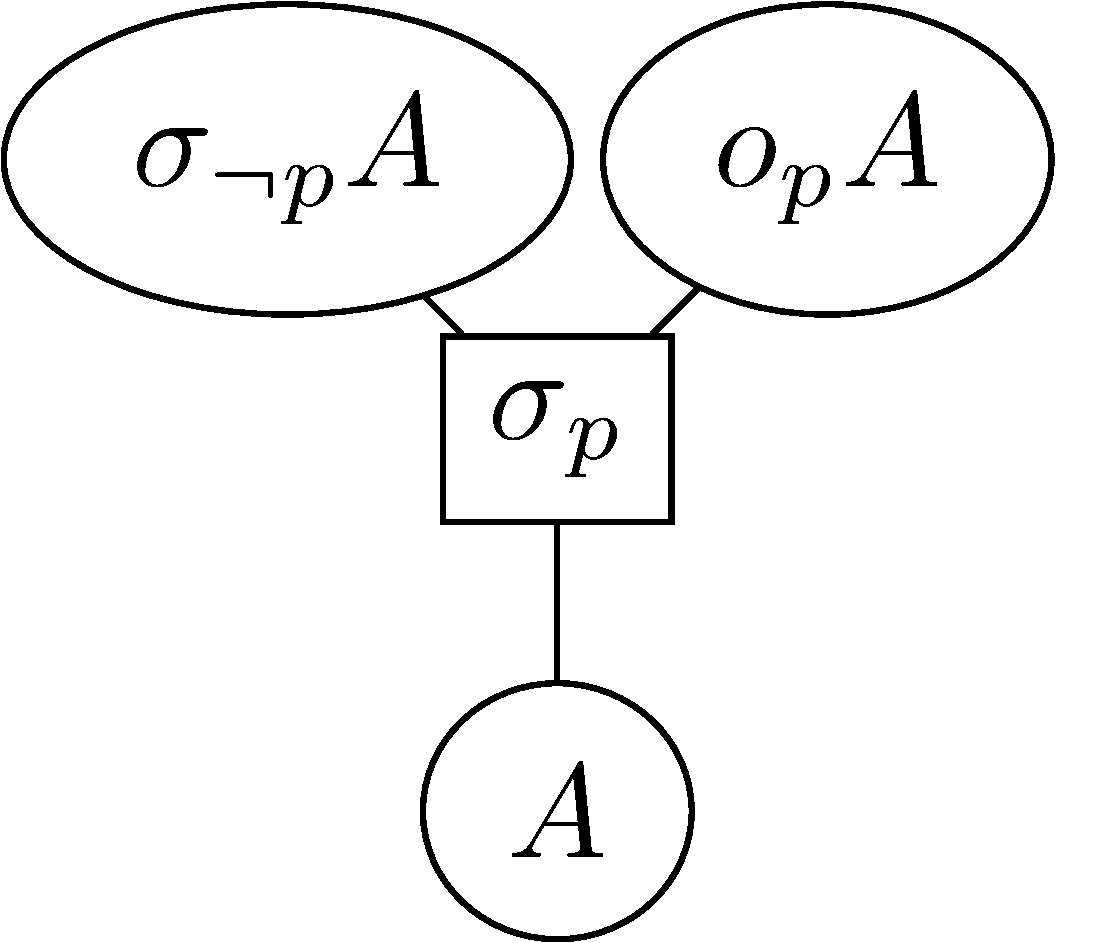
\includegraphics[width=0.3\textwidth]{./imgs/selnet.pdf}
  \caption{\label{fig:org381fe98}A selection t-node may generate both output nodes, rendering it a partition operation.}
\end{figure}

In the figures throghout this work we will denote n-nodes as
circular and t-nodes as squares or rectangles. When materializing
\(\sigma_p(A)\) the planner has the option of also materializing
\(\sigma_{\neg p}(A)\). If deemed beneficial \(A\) can be safely
deleted as the t-node can be reverse triggered to produce it. A
reverse trigger amounts to the union \(\sigma_{p}(A) \cup
\sigma_{\neg p}(A)\). It is generally assumed thoughout this work
that any row not selected by \(p\) is necessarily selected by \(\neg
p\). This means that we do not support missing or NULL values as
they break boolean double negation. Furthermore relations are taken
to be bags of tuples, ie they are unordered.

A slightly more complex example might be

\begin{figure}[p]
  \centering
  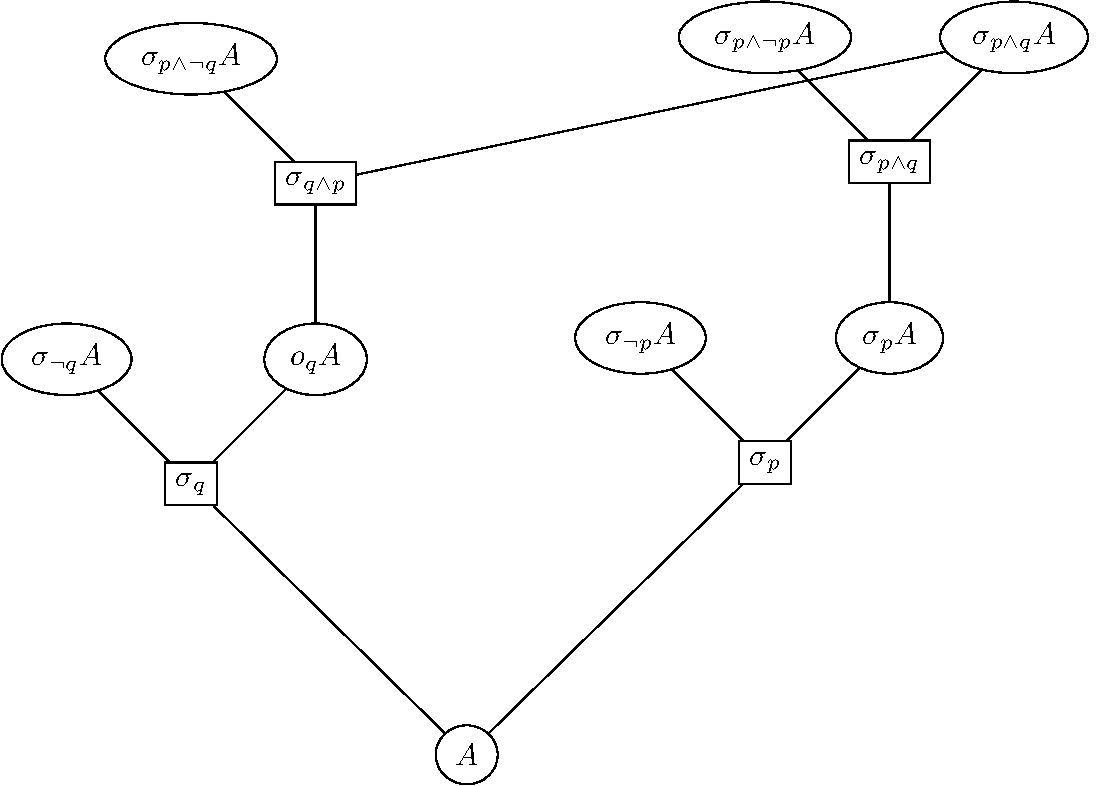
\includegraphics[width=0.9\textwidth]{./imgs/selsub.pdf}
  \caption{\label{fig:orgd6664d1}Multiple captions can be composed to create larger networks.}
\end{figure}

Here if \$$\backslash${\(\sigma\)\textsubscript{\(\neg{}\) p}A,\(\sigma\)\textsubscript{q}\(\sigma\)\textsubscript{p}A,\(\sigma\)\textsubscript{p \(\land\) \(\neg{}\)
    q}A$\backslash$} are all materialized, then \(A\) is materializable as their
union. This way \(\sigma_p\sigma_qA\) is readily available with no space
overhead. Instead the price paied is that in the event that \(A\) is
required in a different context, constructing it requires some
overhead. Furthermore there are two options for materializing
\(\sigma_pA\): either by selecting over \(A\), or via the union
\(\sigma_{q \land p}A \cup \sigma_{\neg q \land p}A\).

We change the nomeclature of the nodes from AND/OR-nodes to t-nodes
and n-nodes, because despite the correspndence between the concepts
and the similarities, as we will see moving forawrd there are major
differences in their functionality. A concept closer to the
functionality of t-nodes and n-nodes, and in fact our very inspiration
for this approach, is \emph{propagators}
\cite{radulPropagationNetworksFlexible2009a}. In short, propagators are
hyperedges in a hypergraph, the nodes of which contain partial
information about a value. Information about a value can be
accumulated from it's neighbors. Each node can obtain at least as much
information about its value as the most precise neighbor. The amusing
yet illustrative example provided in the paper is the one of measuring
the height of a building by means of a barometer. One approach is
timing the barometer's free fall from the top of the building, another
is by measuring the length of the shadow of the barometer and
comparing with the length of the shadow of the building at the same
time of day. One may even use the barometer in it's intended function
and derive the height of by comparing the difference in air pressure
at the roof and at the ground floor. Each of the mentioned methods
will give very noisy or partial information about the magnitude in
question. In the propagator paradigm each of these measurments might
be represended as a node in a hypernet. A propagator edge connecting
these nodes would combine information from all measurements and
improve each of the nodes' accuracy in their perception of the
underlying value. A t-node is similar to a propagator in that it does
not have a strict direction of information flow and can generate
information on either side given information on the other.

Generally there is not an exactly one-to-one corresoncence between
t-nodes and relational operators. Usually that is the case but
there is an exception: the join operator. As we made clear a t-node
can generate any number of its inputs by reverse triggering it as
long as all of the outputs are materialized. Then one approach to
implementing a join operator might be:

\begin{figure}[p]
  \centering
  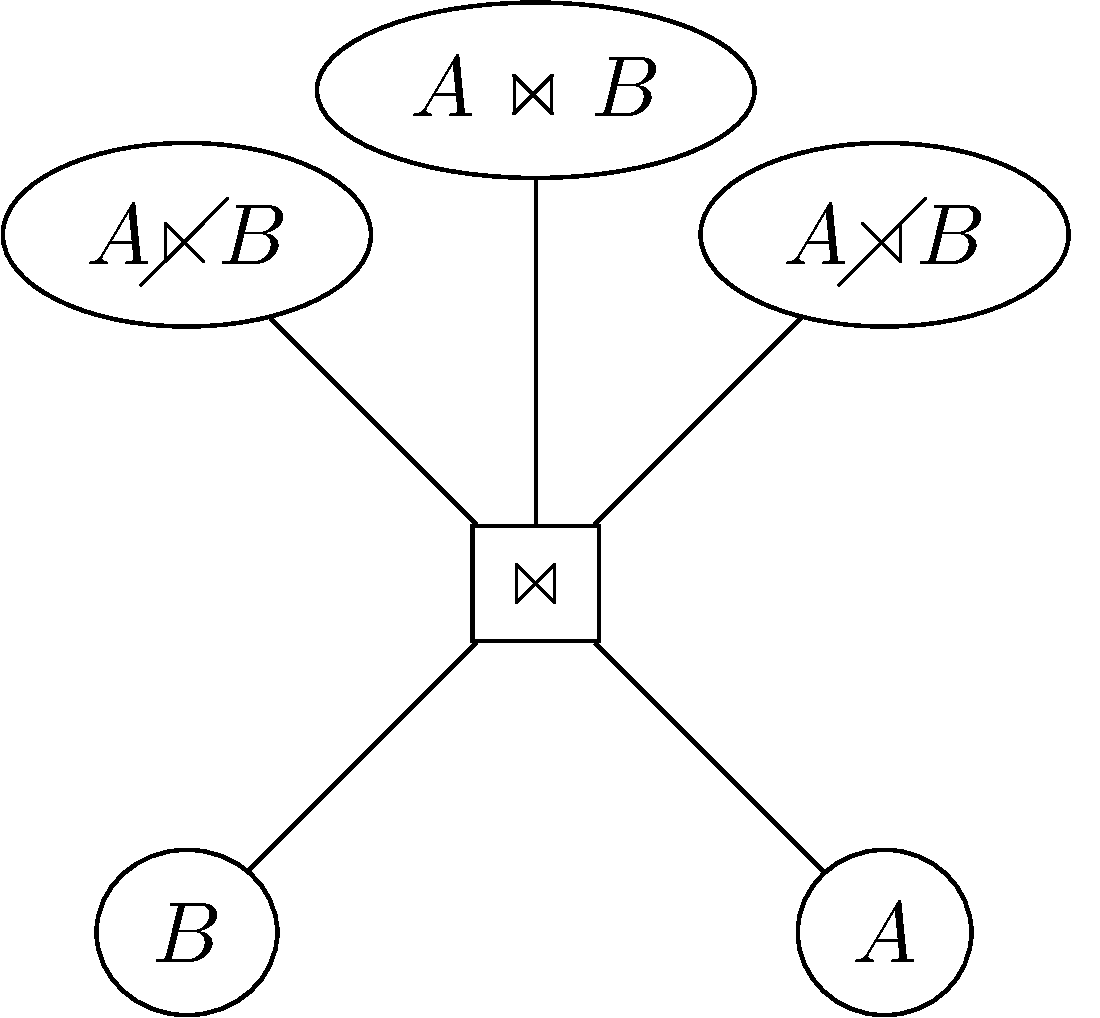
\includegraphics[width=0.5\textwidth]{./imgs/naivejoinnet.pdf}
  \caption{\label{fig:org78bb458}Representing a reversible join as a single t-node.}
\end{figure}


The \(\lnsemi\) operator is the antijoin operator, \(A \lnsemi B\)
includes the tuples in \(A\) that to not participate in \(A \Join B\). It
is the complement of the semijoin \(\lsemi\). Therefore in our
countext

\[ \bar{\pi}_{cols(A)}(A \Join B) \cup (A \rnsemi B) \equiv A \]

We remind the reader that \(\bar{\pi}_{cols(A)}\) means group by the
unique columns of \(A\). Therefore by having materialized \(\{A \rnsemi B, A
\Join B, A \lnsemi B\}\) we can create \({A,B}\) and vise versa. We could,
however be slightly more flexible than that, as we might want to
materialize \(A \rsemi B\) but not \(A \lnsemi B\) to the end of ensuring
the materializability of only \(A\) and not \(B\). We therefore
represent joins not as a single t-node but rather as a cluster of
t-nodes.

However in reality we can afford a bit more flexibility than
choosing between the input and the output sets: We swap \(B \rnsemi A\)
with \(B\) in these sets or \(A \rnsemi B\) with \(A\), thereby having
materialized the tables \(\{A, A \Join B, B \rnsemi A\}\). In this case
neither the entire input nor the entire output are materialized
and yet all tables involved are materializable. To overcome the
limitation that this poses we make the graph a bit more complex
and a bit more flexible by breaking the join into two stages (see
figure \ref{fig:orgceabc4f}):

\begin{itemize}
\item First we separate the join components (\(A\) and \(B\)) into the
  part that will be used in the join (\(A \lnsemi B\) and \(B \lnsemi A\)
  respectively), and the part that will not (\(A \rnsemi B\) and
  \(B \rnsemi A\) respectively).
\item Then we join only the useful parts
  \((A \lnsemi B) \Join (B \lnsemi A) \equiv A \Join B\).
\end{itemize}


\begin{figure}[p]
  \centering
  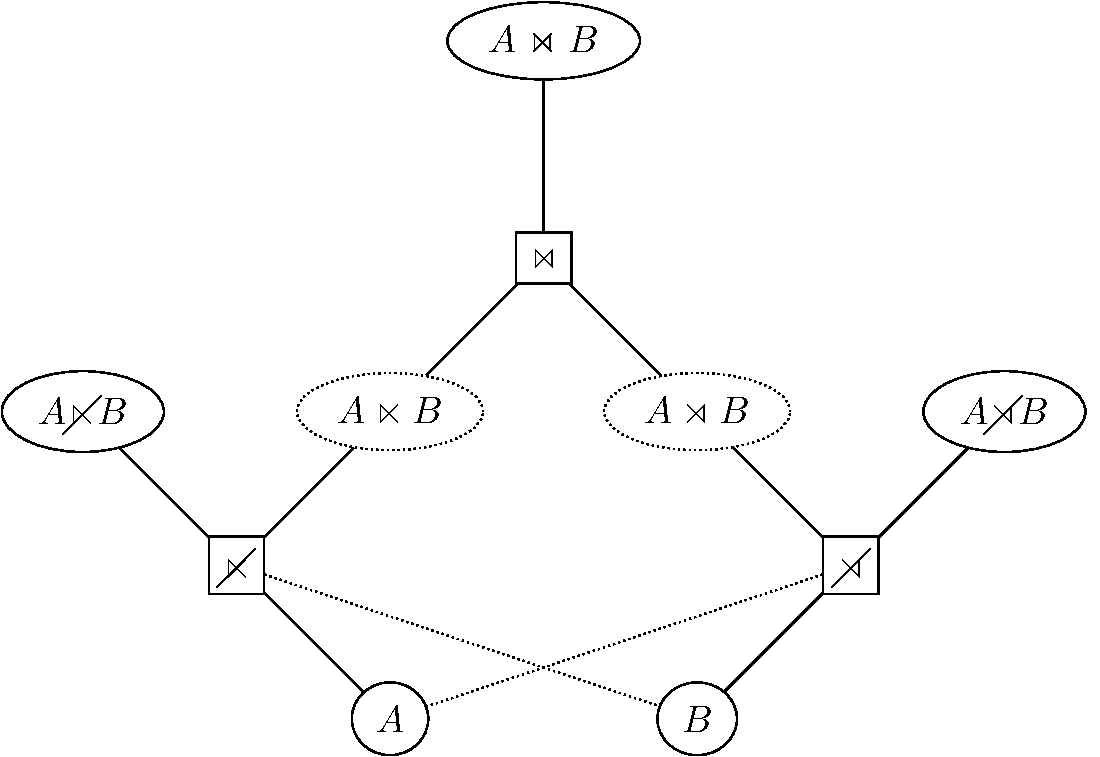
\includegraphics[width=.9\linewidth]{./imgs/joinnet.pdf}
  \caption{\label{fig:orgceabc4f}The DAG corresponding to a join is broken down in multiple t-nodes to facilitate greater flexibility.}
\end{figure}


The left anti-join node partitions \(A\) into \(A \lsemi B\) and
\(A \lnsemi B\), which is left semijoin in our null-less
context. Similarly for the right anti-join node which partitions \(B\) to \(A \rsemi B\) and \(B \rnsemi A\). Joining the semijoin
relations \(A \lsemi B\) and \(B \lsemi A\) is equivalent to
joining \(A\) and \(B\).

In \ref{fig:orgceabc4f} we used an antijoin t-node. From the semantics of the
antijoin \(A \lsemi B\) it is clear that no tuples from \(B\) are
included in either \(A \lnsemi B\) or \(A \rnsemi B\) as \(B\) acts
as a kind of predicate for selecting over \(A\). This means that even
though \(B\) is an input to this there is no natural way of creating \(B\)
from the t-node's output. For these cases we introduce \emph{irreversible
  edges}. Irreversible can only triggered in only one
direction. Remember that edges are always connections between n-nodes
and t-nodes. An irreversible input edge (a connection from an n-node
to a t-node) can only be used as input and its n-node can not be
materialized by reverse triggering the t-node.

Irreversible edges appear in the inputs of anti-join t-nodes but also
on the output of operations that can't be information preserving,
notably aggregations. The output of an aggregation can not in general
be supplemented with extra information to reconstruct the input,
unless the entire input table is replicated. We therefore give up the
reversibility of such operations completely and mark the output edge
as irreversible. This is genrally not a very big problem as on the one
hand the results of aggregations tend to be small compared to the
input relations, and in the case of anti-join t-nodes, which are only
found in join clusters, for every anti-join node \(A \lnsemi B\) that
is unable to generate \(B\) by reverse triggering, there is a \(A
\rnsemi B\) that will happily generate \(B\) albeit refusing to
generate \(A\). This is demonstrated in figure \ref{fig:orgc670489}.

\begin{figure}[p]
  \centering
  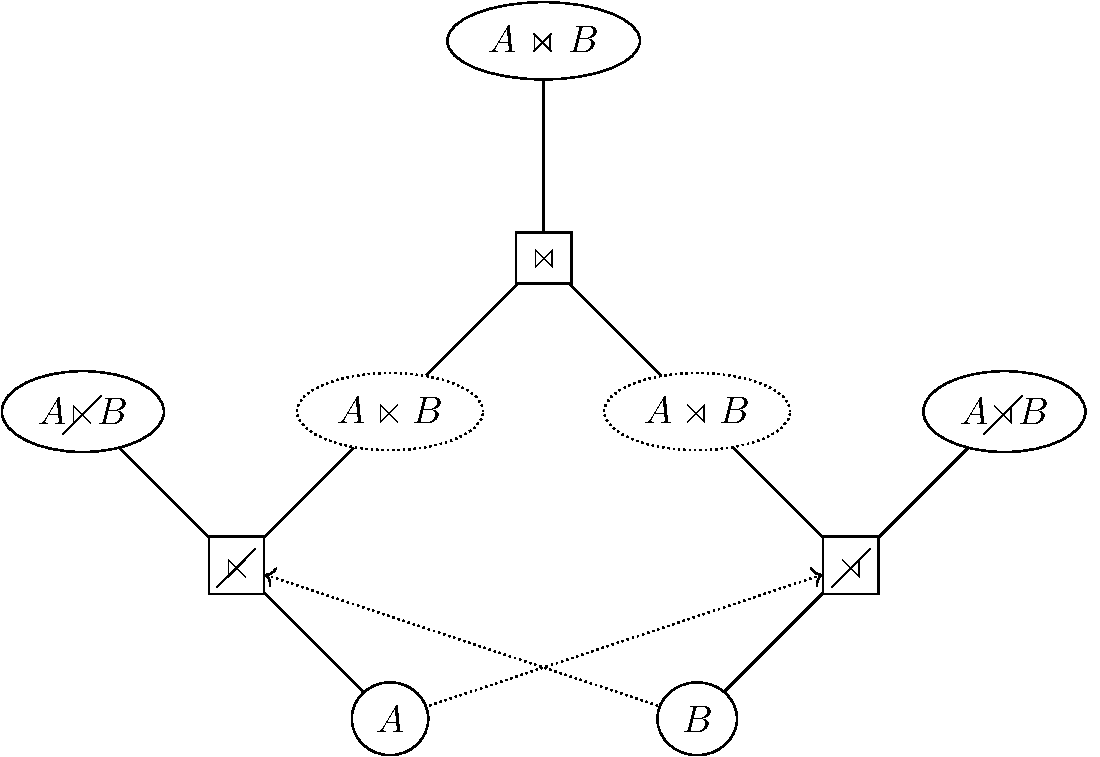
\includegraphics[width=.9\linewidth]{./imgs/joinnetdir.pdf}
  \caption{\label{fig:orgc670489}The DAG corresponding to a join is broken down in multiple t-nodes to facilitate greater flexibility.}
\end{figure}
\section{Deterministic query processing}
\label{sec:orgb65466e}
In this section we will look at the initial steps of what happens when
FluiDB receives a query. Initially the querry is accepted in textual
form as SQL. Then it is sanitized to adhere to the properties we
defined for relational alegbra and some obvious optimizations are
applied to remove artifacts of the parsing process. Finally the query
is translated to a forest if possible join orderings. These are the
rewrite based optimizations that are deterministic and do not take
into account the rest of the workload.

\subsection{Query parsing}
\label{sec:org860b230}
We use a custom library for parsing SQL queries into relational
algebra based on parser combinator monads
\cite{leijenParsecDirectStyle}. Our parser handles both the aprsing and
decorrelation of the queries. In biref, parser combinators is a
functional interface to combining parsers to make larger parsers. A
parser \texttt{p} has the form \texttt{p a} which means that if the parser is used
to parse matching text, it will return a result of type \texttt{a}. For this
framework to work two combinators are required:

\begin{itemize}
\item seqnence (the monadic bind) \texttt{(>>=) : p a -> (a -> p b) -> p b}
  which sequentially tries two combinators and the latter one may use
  the result of the former.
\item the 'alternative' parser combinator \texttt{<|> : p a -> p a -> p a} which
  tries one parser and if that fails tries another.
\item \texttt{MonadGen e p} can generate a value of type \texttt{p e}. Useful for creating
  names for unnamed expressions in projections, groups.
\end{itemize}

Simple parsers like the \texttt{parseInt} parser (listing \ref{org463a483})
combinators are then combined to create more complex parsers (listing
\ref{org39b9e41}). This approach is fundamentally not dissimilar to
writing yacc files but it is much more flexible as it is effectively
an EDSL that inherits all the power of the host language.

\begin{listing}[p]
  \begin{haskell}
    parseInt :: MonadParse p => p Integer
    parseInt = do
    sign <- fmap (maybe 1 (const $ negate 1)) $ parseMaybe $ char '-'
    void $ parseMaybe $ char '-'
    (* sign) . read <$> readWhile isDigit
  \end{haskell}
  \caption{\label{org463a483}A simple parser of an integer}
\end{listing}

\begin{listing}[p]
  \begin{haskell}
    parseSelectProj
    :: (MonadGen e p,MonadParse p) => p e -> p (Query e s -> Query e s)
    parseSelectProj eM = do
    word "select"
    fmap (Q1 . QProj) $ sep1 (word ",") $ do
    ex <- parseExpr (E0 <$> eM)
    parseMaybe (word "as" >> eM) >>= \case
    Just e -> return (e,ex)
    Nothing -> do
    e <- maybe pop (return . mkSymbol) $ asSymbol ex
    return (e,ex)
  \end{haskell}
  \caption{\label{org39b9e41}The selection parser is much more complex and handlse many different cases but it is built up from simple fundamental blocks. This parser returns a query modifier that is meant to be applied a very simple product query generated by the \texttt{from} clause.}
\end{listing}
\subsection{Query preprocessing}
\label{sec:orgd903905}
Immediately after parsing the queries have several potential
inconsistencies with the notion of relational algebra that we
described so far. For that reason we implement an intermediate stage
where we rewrite the query to comply with various properties of the
RA, and which remove redundancies. In brief those are the following:

\begin{itemize}
\item Projections and selections are squashed. For example
  \(\sigma_p\sigma_q\) becomes \(\sigma_{p \land q}\).
\item Date intervals are translated to dates. This is because the plysical
  planner does not handle dates specially so all dates and date
  intervals are converted to timestamps and second intervals. For
  exaple the expression \texttt{date '2020-12-01' - interval '90' day} is
  immediately turned into \texttt{date 2021-03-01}. Note that an expression
  like \texttt{date '2020-12-01' + shipping\_time} is not supported as it is
  not date arithmetic between literals.
\item Optimization of the \texttt{like} operator: \texttt{<VAR> like
    <STRING\_LITERAL>} expressions where \texttt{<STRING\_LITERAL>} begins or
  ends with \texttt{\%} are turned into \texttt{suffix\_of} and \texttt{prefix\_of}
  expressions. For example the expression \texttt{a like "\%.txt"} would be
  turned into \texttt{".txt".suffix\_of(a)}.
\item Substring expressions are turned into 0-indexed ones from
  1-indexed as is the case in SQL.
\item It is asserted that each intermediate relation has uniquely named
  columns. For example there are necessarily name conflicts in \(A
  \Join A\).
\item It is asserted that sorting appears higher in the query AST than a
  selection, a join or an aggregation. All three of these operators
  affect the ordering of their inputs (see chapter 4 on code
  generation), and sort is the only operation that asserts tuple
  ordering on its output. Therefore \(s(A \Join B)\) is valid but
  \(s(A) \Join B\) is not.
\end{itemize}

Once the preliminary sanitization and simple optimization steps are
done we mark each instance of the primary table symbols with the
columns and their types. This is simply information derived by the
databse schema. Then we do some processing and annotation on symbols
referring to symbols:

\begin{itemize}
\item First \emph{remap unique sub-tuples}. Each intermediate result, and each
  relation that we want to be able to reason about needs to have
  uniquely identifiable rows. For each relation in the QDAG we are
  keeping track of a set of columns, the unique sub-tuple, the
  combination of which is unique among the tuples of the same
  table. It is fairly easy to keep track of the unique subtuple for
  most operations, e.g. the unique sub-tuple of a cartesian product or
  join is generally the concatenation of the unique sub-tuples of the
  input tables, the unique sub-tuple in the case a selection is the
  same as the unique sub-tuple of the input, in aggregations the
  unique sub-tuple is the same as the columns on which we aggregate,
  etc. The main problem is projections and, in a similar manner
  aggregations, where it is possible that the operation does not
  project on the entire unique sub-tuple. To mitigate this we perform
  a pre-processing setp to rewrite the projections to expose the
  entier unique sub-tuple. It is worth mentioning that there are cases
  where there are more than one combinations of columns that form a
  unique sub-tuple. We opt to keep track of all of them in order to
  have more flexibility in this pre-processing step: ideally we want
  to modify the projection as little as possible. In other words we
  want to project as few extra columns as possible to keep the table
  size as small as possible.
\item annotate each symbol refering to a column with the corresponding
  primary table if there is one (named columns of projections do not
  correspond to a primary table)
\item Infer and annotate the type of each column referene.
\end{itemize}


\subsection{Possible joins}
\label{sec:org2eb887b}
The focus of our optimization where we separate different plans of the
query where it is a-priori unclear which of them is the optimal, much
less which is the optimal accounting for generated intermediate
views. We focus on enumerating all possible join permutations. First
all joins are turned into selection-products so \(A \Join B\)
becomes \(\sigma(A \times B)\), selections are pulled up and merged
(\(\sigma_p \sigma_q A\) becomes \(\sigma_{p \land q}\)) and
products are represented as sets of relational algebraic
expressions. Then all possible permutations of joins are created. For
example \(\sigma{a=b \land b=c}(A \times B \times C)\) becomes \(\{(A \Join_{a=b} B) \Join_{b=c} C, A \Join_{a=b} (B \Join_{b=c} C)\}\). Note that we do not include queries that are only different
w.r.t. commutativity, ie we don't include both \(A \Join B\) and \(B \Join B\), this part of FluiDB depends on the consumer of the data
structure to disambiguate between them. Also note that since cartesian
products are very large and almost never used in the actual plans, an
option that disallows product intermediate results is enabled by
default. Therefore, in our example we do not enumerate relations like
\(\sigma_{a=b}((A \times C) \Join_{b=c}B)\). Furthermore, allowing
cartesian products exponentially explodes the space of possible plans
and makes the results unusable.

Once selections are merged we find product trees, i.e. contiguous parts
of the tree that only contain cartesian products, and combine them
into multisets of subtrees such that \(\sigma(C \times (A \times B)
\times D)\) becomes \(\sigma(\{A,B,C,D\})\). Then selection propositions
are normalized to conjunctive normal form and into sets. For example
\(\sigma_{p_1 \lor (p_2 \land p_3}A\) becomes \(\sigma_{(p_1 \lor p_2)
  \land (p_1 \lor p_3)}A\), and in fact the conjunctive terms are also
represented as sets of subterms, so the final form would be better
expressed as \(\sigma_{\{p_1 \lor p_2,p_1 \lor p_3\}}A\). This leaves us
with a tree of terms of the form
\(Q[\sigma_{\{p_0,p_1,...,p_l\}}\{Q_0,Q_1,...,Q_k\}]\) where each term
\(p_i\) refers to columns in one or more \(Q_j\) relations and
\(Q[\cdot]\) is a query tree with \(\cdot\) as a subtree. We will
refer to such a selection-product pair as an SP-term.

To turn this representation into a forest we will turn each SP-term
into a set of regular join trees, the cartesian product of which will
yiled the possible joins. We summarize the process as follows:

\begin{itemize}
\item We iterate over all the pairs of multisets into which the multiset
  \(\{Q_0,Q_1,...,Q_k\}\) can be split. We follow each of the
  following steps for each of the multisets.
\item we split the \(p\) terms in three parts depending on which
  sub-multiset of relations their symbols refer to. One set are terms
  where the columns mentioned refer \emph{only} to the left sub-multiset
  (left \(p\)-terms), another set are terms where columns mentioned
  refer \emph{only} to the right sub-multiset and the rest (right
  \(p\)-terms) must necessarily have references to columns of \emph{both}
  sub-multisets. We call the latter category \emph{connector \(p\)-terms}.
\item We turn each side of the split into an SP-term by associating it
  with the left and right \(p\)-term set. We recursively repeat the
  process of generating join trees out of each SP-term created and
  connect them in an all-to-all fashion by creating theta joins using
  the conjunction of the connector \(p\)-terms. In case the the set of
  connector \(p\)-terms is empty that would mean that the connection
  of the join trees must be done with a cartesian product. As
  mentioned above we want to avoid inserting cartesian products in our
  graph so we reject those cases outright. Optionally we may even want
  to reject all non-natural joins altogether, unless that would mean
  not coming up with any plans at all.
\end{itemize}


It is worth mentioning that an issue with this approach is the
handling of projections. As elaborated in the section on \hyperref[sec:org860b230]{query parsing}
projections come up a lot in decorrelating queries. Joins separated by
projections can not trivially be mixed with the above method as moving
projections would potentially break the rule that we demand that there
is no naming conflict between columns. Even though as things stand
this case is not handled our method of uniquifying columns is powerful
enough that the non-conflict rule could potentially be relaxed by
applying methods similar to the ones we deploy in disambiguating
columns section on \hyperref[sec:org9e7f455]{Query Normal forms (QNF)}.

The fundamental forest structure of literally collecting each logical
plan individually is highly redundant. Therefore, we abstract away the
redundancy by representing the forest as a bipartite tree.

\begin{itemize}
\item One kind of node represents a plan fragment. We will refer to
  these as sub-trees.
\item The other kind represents a forest of semantically equivalent
  subtrees earmarked with a unique hash for them. The fact that the
  subtrees are semantically equivalent means that they essentially
  evaluate to the same data. They therefore have the same normal form
  as discussed in Query Normal forms (QNF, see section [ref]). Finding
  the normal form hash of one would mean the normal form hash of the
  rest. This will prove useful when inserting this structure in the
  graph. We refer to these as sub-forests.
\end{itemize}

In other words the relational algebra tree is interleaved with
OR-nodes of different representations of the subquery. For example
\(\gamma(\sigma_{a=b \land b=c}(A \times B \times C))\) becomes
\(\gamma\{A \Join_{a=b} B) \Join_{b=c} C, A \Join_{a=b} (B \Join_{b=c}
C)\}\). This way we avoid the compinatorial explosion of interleaved
nesting joins with other operations.

The algorithm is also described in listing \ref{org9aea439}.

\begin{listing}[p]
  \begin{minted}[]{python}
    def possible_joins(q):
    # Split a query that is equvanent to
    # sel(p1 and p2 and p3 and ..., prod(q1, q2, q3,...))
    # into
    # [p1,p2,p3,..], [q1,q2,q3,...]
    and_props,subqueries =  as_prod(q)

    # If there are no top level joins traverse the query
    if len(and_props) == 0:
    return q.map_children(possible_joins)

    # All possible partitions where the partitions are non-empty
    for lqs,rqs in possible_partitions(subqueries):
    # has_free_vars(p,[q1,q2,q3...]) checks if all the atoms in p
    # are either literals or columns in one of the q1,q2,...
    lps = filter(lambda p: not has_free_vars(p,lqs), and_props)
    rps = filter(lambda p: not has_free_vars(p,rqs), and_props)
    # The props thet connect the partitions into a join.
    jps = filter(lambda p: has_free_vars(p,lqs)
    and has_free_vars(p,rqs),
    and_props)
    # If there are no predicates connecting it is product. We
    # disallow products.
    if len(jps) == 0: continue
    # A valid join to be considered while planning!
    lq = sel(lps,prod(rqs))
    rq = sel(rps,prod(rqs))
    yield join(jps,possible_joins(lq), possible_joins(rq))
  \end{minted}
  \caption{\label{org9aea439}Pseud-python description of finding all possible for clarity it is abreviated to omit sanity checking, memoization, some type conversions, etc.}
\end{listing}

It is worth mentioning that as many of the subtrees generated this way
will be equivalent. As analyzed in
\cite{selsamSealingPointerbasedOptimizations2020} and discussed in
section g in pure functional settings like ours DAGs can
have explosive complexity during traversal. Even worse in this case
even the space complexity can indeed be needlessly exponential. For
that reason we maintain a hash map matching hashes with the
corresponding matching subtrees. Before inserting a newly created
forest into our tree we perform a lookup in the hash map. If we find
something we throw away the newly created forest for the garbage
collector to recycle and use the one in the hash map
instead. Otherwise we insert our forest both in the hashmap and in the
tree. This way we deduplicate our data structure. Furthermore, in the
same vain as \cite{selsamSealingPointerbasedOptimizations2020} we
earmark all our forests with their hash so we don't have to traverse
them again to compute it. The result of this is that in total we
completely traverse the forest once to compute the hashes of each
sub-forest and then we use those hashes to test sub-forests for
equality.




\section{Section: Query Normal forms (QNF)}
\label{sec:org9e7f455}
It is imperative that the QDAG has as little redundancy as possible,
two subqueries that descibe the the same relation should be
represented as the same node. Equivalence of RA expressions is
infamously NP-complete
\cite{sagivEquivalencesRelationalExpressions1980} but we make a best
effort to normalize queries such that they are hashable and comparable
via simple structural equality. The core of normalization is
transforming the queries to cartesian normal form

\[
  \zeta_{x_1}(A) \Join_{p_1} \zeta_{x_2}(B) \Join_{p_2} \zeta_{x_3} (\sigma_{p_3}(C)) \to \zeta_{x_1;x_2;x_3}(\sigma_{p_1 \land p_2 \land p3}(A \times B \times C))
\]

where \(\zeta \in \{\pi,\gamma\}\).


\subsection{QNF Structure}
\label{sec:org1912b6b}
Query Normal Forms is a highly polymorphic datastructure separate from
the the \hyperref[sec:relational_algebra_semantics]{RA} data structures, which in its general form encapsulates one
of several special forms, all of which strive to abstract away as many
rewrites as possible, and ideally achieve a one-to-one correspondence
between a QNF and a table. The QNF in its general form (listing
\ref{org4e7446e}) is specialized to represent several different forms
internally to the QNF subsystem, outside of it there are two main
objects:

\begin{itemize}
\item The normal form of a query
\item A column of a normal-form query.
\end{itemize}

\begin{listing}[p]
  \begin{haskell}
    data QNFQuerySPDCF sel_f prod_f dbg_f col_f f e s =
    QNFQuery
    { qnfColumns :: col_f (QNFProj f e s) (QNFAggr f e s)
      -- ^ What columns kept. Each of these is a column on one of the
      -- QNFProd.
      ,qnfSel :: sel_f (QNFSel e s)
      -- ^ And conjuction of selection. The QNFNames here lack a qnfProd
      -- and qnfSel because they are names of this QNFQuery itself so to
      -- avoid a recursive structure that we need to keep up to date we
      -- just promise that they will be empty.
      ,qnfProd :: prod_f (QNFProd e s)
      -- ^ QNFProd e s refers to multiple rewrites of a single
      -- relation. Essentially {Query (..) (QNFQuery e s)}. Each element
      -- of this set needs to have the same set of QNFQuery's. The binary
      -- operators allowed here MUST expose plans from ONE side. Otherwise
      -- the qnfColumns will be ambiguous. In practice only Product/Join
      -- expose both sides but if there are more in the future know that
      -- qnf machinery will break.
      ,qnfOrigDEBUG' :: dbg_f (Query e s)
      ,qnfHash :: QNFKey e s
      -- ^ Cache the hash. Hashing is done separately for each field so we
      -- don't recompute hashes of unchanged fields after each operation.
    }
  \end{haskell}
  \caption{\label{org4e7446e}The QNF datastructure.}
\end{listing}


We depend to distinguish between different queries and to recognize
equivalent queries. In the section on building QNFs we will look at
several specializations that are useful as intermediate. In this
section we will focus on each of the fileds of the \texttt{QNFQuery}
constructor.
\subsubsection{QNF Columns, projections and aggregations}
\label{sec:orgba02a81}
Whenever a \texttt{QNFQuery} is found outside of the QNF package \texttt{col\_f} will
be instantiated as \texttt{Either}, which is to say that a query may be an
aggregation (\texttt{Right}) or a projection (\texttt{Left}). When there is no
explicit projection at the top of a query, the columns are simply
enumerated. While the \hyperref[sec:relational_algebra_semantics]{RA} is fundamentally named, \texttt{QNFQuery} instances
are unnamed. Instead we use a \texttt{QNFColumn} in place of names. With that
in mind, we define the projection operator as an unordered bag of
expressions.

\begin{listing}[p]
  \begin{haskell}
    type QNFProj f e s = f (Expr (QNFName e s))
  \end{haskell}
  \caption{\label{orgcefa865}A QNF projection field is a collection of expressions that refer to QNF names. The particular structure of this collection is parametric. When the collection \texttt{Identioty} the QNF query is essentially just a column. A normal QNF query would instantiate \texttt{f} to \texttt{HashBag}, an unordered multiset.}
\end{listing}

Before getting into detail about \texttt{QNFName}, we need to make clear that
depending on the instantiation of \texttt{f} we get different structure in
the project. When \texttt{f \textasciitilde{} Identity} the projection set only contains one
element and the QNF is essentially a column. Indeed this is exactly
how we define columns and on that we build to define names (see
listing \ref{org0b2230d}). An name in the context of QNFs refers to an
exprsssion atom which can be one of three different kinds:

\begin{itemize}
\item A column of a non-primary relation. This relation \textbf{must} be a member
  of the product collection. Because there may be more than one
  equivalent queries ion the product collection we index the columns
  with an integer.
\item A column of a primary table. These columns have a name and are
  associated with a table (\texttt{s}) which needs to be in the product
  collection like in the case of non-primary columns. It is indexed
  much like the non-primary relation.
\item A non-column (non-symbol) name, i.e. a literal is also a QNF name.
\end{itemize}

The column of a non-primary relation as mentioned is nameless. It is
simply a the relation itesf with the rest of the columns removed. We
ensure that by using the \texttt{Identity} functor as the container for the
projection columns (see listing \ref{org0b2230d}).

\begin{listing}[p]
  \begin{haskell}
    data QNFNameSPC sel_f prod_f col_f e s
    = PrimaryCol e s Int
    | Column (QNFColSPC sel_f prod_f col_f e s) Int
    -- ^ a a column c that refers to a:
    --
    -- QNF[P[c],S[c],Prod[Query[a ~ QNF]]]
    | NonSymbolName e
    -- ^ A literal.

    -- A column is a QNF that has one element in the projection set
    -- (Identity) and no debug query.
    type QNFColSPC s p c = QNFQuerySPDCF s p EmptyF c Identity
  \end{haskell}
  \caption{\label{org0b2230d}A QNF name may be an unnamed column of a relation, a named column of a primary table or a literal.}
\end{listing}

In listing \ref{orgcefa865} we see the definition of the projection field
of the QNF. It mirrors the structure of a projection like the ones we
saw in the section where we decribed the \hyperref[sec:relational_algebra_semantics]{RA} but unnamed and without
any ordering. The \texttt{Expr} however is the same. FluiDB makes no attempt
to normalize the expressions so equivalent expressions that differ
syntactically will produce different QNFs.

As mentioned the columns in the QNF name, both primary and of general
relations, are indexed in the case that there are more than one
equivalent. This is an edge case that can cause problems because
different indexing can cause equivalent nodes to have different
syntactic representations. The query \texttt{select * fom A as A1, A as A2
  where A1.a = A2.a} is symmetric in all repsects but the query
\texttt{select * fom A as A1, A as A2 where A1.a = A2.a + 1} is not. Indexing
\texttt{A1} and \texttt{A2} differently does not change the semantics of the query
but it changes the QNF representation. This is not commonly a problem,
a rare edge case rather, but it is a problem nontheless. In an attempt
to mitigate this we generate \textbf{all} different combinations of indexing
are emitted by the \hyperref[sec:org3f1036f]{QNF builder}. In that section we discuss in detail
how that is done in FluiDB.

Very similar to projections are aggregations (listing
\ref{org3c5bf71}). However they only operate on the non-recursive \texttt{Aggr}
algebra, while \texttt{QGroup} uses \texttt{Expr (Aggr (Expr e))}. QNF moves the
inner and outer \texttt{Expr} to one level up and one level down
respectively, so an aggregation \(\gamma S\) would be rewritten to an
equivalent \(\pi \gamma \pi S\).

\begin{listing}[p]
  \begin{haskell}
    type QNFAggr f e s =
    (f (Aggr (QNFName e s)),HS.HashSet (Expr (QNFName e s)))
  \end{haskell}
  \caption{\label{org3c5bf71}The QNF aggregation form of the projection field is similar to projection only, much like the \texttt{QGroup} constructor, it also includes a hashset of exprssions on which to group.}
\end{listing}

\begin{enumerate}
\item Named QNFs
  \label{sec:orge07cacb}

  As stated in the previous section QNFs are fundamentally unnamed with
  the exceptions of primary columns and indexes. However, there are
  occasions where we want to refer to columns of a QNF by the name of
  the RA expression based on which it was created. One example is while
  \hyperref[sec:org3f1036f]{building QNFs} where given an expression \(\sigma_p A\) we first
  translate \(A\) to QNF. To proceed need a way to relate the symbols
  appearing in \(p\) with the columns of \(A\). To mitigate this define
  a \emph{named QNF} which is simply a tuple of a QNC along with a mapping
  between symbols and columns of that QNF (see listing \ref{org23a05f8}).

  \begin{listing}[p]
    \begin{haskell}
      -- | col_f is Const for Projections, CoConst for aggregations and
      -- Either for any of the two. We instantiate the collection holding
      -- the columns of the QNF as Identity to indicate that the QNF has one
      -- column and is therefore ... a single column.
      type QNFColC col_f = QNFQueryCF col_f {- f: -} Identity
      -- | The name map is simply a mapping between names of type e and
      -- columns.
      type NameMapC c e s = HM.HashMap e (QNFColC c e s)
      -- | An NQNF is as parametric as a normal qnf but it name
      -- annotatations for the columns.
      type NQNFQueryDCF d c f e s = (NameMapC c e s, QNFQueryDCF d c f e s)
    \end{haskell}
    \caption{\label{org23a05f8}A named QNF is a QNF along with a map that allows us to relate the QNF columns with the symbols used by the RA expression on which it was based.}
  \end{listing}
\end{enumerate}


\subsubsection{Named QNFs}
\label{sec:org0612bfe}
As stated in the previous section QNFs are fundamentally unnamed with
the exceptions of primary columns and indexes. However, there are
occasions where we want to refer to columns of a QNF by the name of
the RA expression based on which it was created. One example is while
\hyperref[sec:org3f1036f]{building QNFs} where given an expression \(\sigma_p A\) we first
translate \(A\) to QNF. To proceed need a way to relate the symbols
appearing in \(p\) with the columns of \(A\). To mitigate this define
a \emph{named QNF} which is simply a tuple of a QNC along with a mapping
between symbols and columns of that QNF (see listing \ref{org23a05f8}).

\begin{listing}[p]
  \begin{haskell}
    -- | col_f is Const for Projections, CoConst for aggregations and
    -- Either for any of the two. We instantiate the collection holding
    -- the columns of the QNF as Identity to indicate that the QNF has one
    -- column and is therefore ... a single column.
    type QNFColC col_f = QNFQueryCF col_f {- f: -} Identity
    -- | The name map is simply a mapping between names of type e and
    -- columns.
    type NameMapC c e s = HM.HashMap e (QNFColC c e s)
    -- | An NQNF is as parametric as a normal qnf but it name
    -- annotatations for the columns.
    type NQNFQueryDCF d c f e s = (NameMapC c e s,QNFQueryDCF d c f e s)
  \end{haskell}
  \caption{\label{org68b5d7d}A named QNF is a QNF along with a map that allows us to relate the QNF columns with the symbols used by the RA expression on which it was based.}
\end{listing}


\subsubsection{QNF Selection}
\label{sec:org4074deb}
The \texttt{qnfSel :: sel\_f (QNFSel e s)} field contains an exprssion of the
selection (see listing \ref{orgc76c888}). With very few exceptions \texttt{sel\_f}
is instantiated as an unoredered hash which is conjoined.

\begin{listing}[p]
  \begin{haskell}
    type QNFSel e s = Prop (Rel (Expr (QNFSelName e s)))
  \end{haskell}
  \caption{\label{orgc76c888}Selection name refers to a version of the current QNF that has all fields erased except the projection.}
\end{listing}

Selection names refer to the \emph{output columns} of the QNF which makes
the QNF implementation would be self referrential. Therefore we drop
the selection and product info aspect from all symbols in
\texttt{qnfSel}. This way we can update the fields of the QNF without needing
to keep the columns in sync with the columns referenced in
\texttt{qnfSel}. This eliminates the need for both indexing the columns and
for dealing with primary colmns in \texttt{QNFSelName}. This has to do with
the way selections are being created: the RA expression \(\sigma_p A\)
is translated by first translating \(A\) to a named QNF. Then \(p\)
refers directly to the columns of the query.

It needs to be pointed out that \emph{despite} the fact that the \texttt{qnfSel}
field refers to output columns the order of operations in the sematics
of a QNF is \(\pi\sigma(..)\) rather than \(\pi\sigma(..)\). In the
case where \texttt{cnfCol} describes a projection the selection can be pushed
down. In the case, however, where \texttt{cnfCol} describes an aggregation
things are more complicated. We will get into this more when we
describe the \hyperref[sec:org3f1036f]{QNF computation}, for now suffice it to say that a new QNF
projection layer is created to accompodate this case.

We generally do not do any normalization of expressions or predicates
beyond turing \texttt{Prop} into a unordered \(\land\)-set with one
exception: ordering the sides of equalities. Equality relations are
flipped if necessary so that all subexpressions \(E_0 = E_1\) in a QNF
have \(hash(E_0) \le hash(E_1)\).


\subsubsection{QNF Product collection}
\label{sec:org86e5e2d}
The \texttt{qnfProd :: prod\_f (QNFProd e s)} field contains the
unordered collection of subqueries \(\{A_1,... , A_n\}\) in the
equivalent \(\pi \sigma (A_1 \times ... \times A_n)\), typically as a
hash-set (via the instantiation of \texttt{prod\_f} as
\texttt{HashSet}). The \(A_i\) of a QNF \(Q\) terms may be one of the
following:

\begin{itemize}
\item Primary tables
\item QNFs with an opposite kind \texttt{qnfCol} (if \(Q\) is a projection an
  \(A_i\) may be an aggregation)
\item A set of equivalent RA expressions that are not reducible to the
  \(\pi \sigma(A_1 \times ... \times A_n\).
\end{itemize}

Focusing on the latter case, there are certain equivalent rewrites
that are not easily expressible in the QNF. For that reason instead of
perpetually extending the QNF system we provide this expensive method
of simply enumerating equivalent queries in RA form. These RA queries
have at the leaves of the expressions either QNFs or primary
tables. The only restriction that we place on these queries is that
the schema of the inputs is simply forwarded to the output without
modification of the individual fields so that the \texttt{cnfCol} vector can
refer directly to them.

\begin{verbatim}
\pi(...,1+a,...) {
  \sigma(...) {
    ... \times (B \triangleleft A) \times ...
  }
}

a is a column of A
\end{verbatim}


\subsubsection{QNF Misc fields and hashing}
\label{sec:org74a3a45}
There are two more fields in the generic QNF datastructure we
described. \texttt{qnfOrigDEBUG' :: dbg\_f (Query e s)} is the more
straighforward one. It simply keeps track of the query used to create
the QNF for debugging puproses. Therefore, \texttt{dbg\_f} is typically
instantiated to \texttt{EmptyF} in practice to save on memory.

The other datastructure is the \texttt{qnfHash :: QNFKey}. Because the QNF is
a highly self referrential data structure equality in a purely
functional environment like Haskell is a very expensive operation. For
that reason in practice we depend on hashes to detect equivalence. As
te QNF has three distinct parts that are being often updated during
building of a QNF (see listing \ref{orgabd13d0}).

\begin{listing}[p]
  \begin{haskell}
    type QNFKey e s = (Int,Int,Int)
  \end{haskell}
  \caption{\label{orgabd13d0}A key that uniquely idnetifies a QNF.}
\end{listing}

Since QNFs are rarely used as anything other than a token for relating
RA form queries FluiDB save on memory and use \texttt{QNFKey} in place of the
\texttt{QNFQuery} structure (see listing \ref{org491a01e}). On the other hand,
in a more pedantic but correct mode, we can avoid depending on the
quality of the hash function and define equality as recursively
checking between all types (see listing \ref{org4097f67}). In
practice we have never found the former method to yield a false
positive for equality.

\begin{listing}[p]
  \begin{haskell}
    instance Eq (QNFQuerySPDCF sel_f prod_f d col_f f e s) where
    x == y = qnfHash x == qnfHash y
  \end{haskell}
  \caption{\label{org491a01e}A fast and loose definition of equality between QNFs that depends on the quality of equality.}
\end{listing}

\begin{listing}[p]
  \begin{haskell}
    instance Eq (QNFQuerySPDCF sel_f prod_f d col_f f e s) where
    x == y = qnfProd x == qnfProd y
    && qnfSel x == qnfSel y
    && qnfColumns x == qnfColumns y
  \end{haskell}
  \caption{\label{org4097f67}A very inefficient but correct equality between QNFs.}
\end{listing}




\subsection{QNF Computation}
\label{sec:org3f1036f}
In this subsection we will look at a few parts of the QNF building
process that are maybe less than obvious. The entire process of
computing QNFs works within a monad stack with the following features:

\begin{itemize}
\item A \texttt{ListT} allows for non-deterministic computation in order to
  account for the different possible column index assignemnts
  described in the subsection on \hyperref[sec:org86e5e2d]{QNF Product collection}.
\item Mutable state that facilitates caching. Since the resulting QNF is a
  highly self referrentlial structure, it is to be expected that a lot
  of the computation might be duplicated. The cache object is also
  shared between different QNF building processes that we know have a
  lot of overlap, for example when inserting nodes into the graph
  without shared caching FluiDB would be repeatedly computing the QNF
  of the same RA subqueries.
\item The process of building a QNF can fail when processing malformed RA
  forms.
\end{itemize}

The types relevant to the computation are presented in listing
\ref{org1fad8c0}

\begin{listing}[p]
  \begin{haskell}
    -- | The monad in which coimputation happens. Not all transformations
    -- require non-determninsm.
    type QNFBuild0 e s = StateT (QNFCache e s) (Either (QNFError e s))
    type QNFBuild e s = ListT (QNFBuild0 e s)
  \end{haskell}
  \caption{\label{org1fad8c0}QNF computation monad provides non-determinism, caching, and error handling.}
\end{listing}

Every QNF building function returns an \texttt{NQNFResult} (listing
\ref{orgd85408f}) contains

\begin{itemize}
\item An operator with the expression atoms translated to QNF names
  refering to the input or output columns depending on the particular
  operator. For example if the operator is a selection all atoms, in a
  projection map the left hand side atoms of the projection are output
  columns and the right hand side atoms are QNF columns that refer to
  the inptu QNF. This is for convenience so that assumes that the RA
  query that was just normalized is a logical plan. The top level
  operator can then be used to annotate QDAG elements that relate to
  the normalized query. The importance of this is analyzed in depth in
  the section on \hyperref[sec:orgcc899ec]{symbol corresponcence}.
\item A mapping between input and output QNF columns.
\item A  named QNF which is the main payload of the QNF building function.
\end{itemize}

\begin{listing}[p]
  \begin{haskell}
    data NQNFResultDF d f op e s =
    NQNFResult
    { nqnfResNQNF :: NQNFQueryDCF d Either f e s
      ,nqnfResOrig :: op
      -- Map the names exposed by the input qnf to names on the output
      -- qnf. Unless qnfResOp is QProj, QGroup each input name corresponds
      -- to 0 or 1 name in the output. So if qnfResOp is QProj or
      -- qnfResInOutNames has no meaning and will be `const Nothing`
      ,nqnfResInOutNames :: [((e,QNFCol e s),(e,QNFCol e s))]
    }
  \end{haskell}
  \caption{\label{orgd85408f}The internal QNF building functions provide some more information that was created during the generation of the QNF, precicely a name map relating column names to QNF names,  a map relating input qnf names to output QNF names, and the top level operator with the names translated appropriately to input or output QNF names.}
\end{listing}

The way most QNF functions are implemented is fairly straighforward,
with the possible exception of products. In the case of looking for
the product of two named QNFs \(Q_1\) and \(Q_2\).  Look for conflicts
where columns of \(Q_1\) can be found in the product collection of
\(Q_2\) and increment their index. Then do the same in reverse and
provide both results as branches of the non-deterministic monad
\texttt{ListT}. So for example if we want find the product
\(\sigma_{a_0=1}(A_0) \times \sigma_{a_0=2}(A_0)\) we get in QNF-like
form \(\sigma_{a_0=1 \land a_1=2} (A_0 \times A_1)\) and also
\(\sigma_{a_1=1 \land a_0=2} (A_0 \times A_1)\)


\subsection{Symbol correspondence}
\label{sec:orgcc899ec}
The schema of each n-node is described in terms of column IDs that are
agnostic to the particular name assigned to it by the user. Therefore
the first step before inserting an operator in the graph is to
normalize the symbol name. We consider that two symbols are equal only
if they refer to the exact same column. This is done by means of
converting the query into normal form. This is required to resolve the
possible ambiguity of symbols with the same name but different scope
when expressions are moved around. This abstracts away the symbol
names but creates some complications. In the query \(\sigma_{a=x \lor
  a=z}(\gamma(\sigma_{a<y}(A))\) the \(a\) in \(a=x\) and the \(a\) in \(a < y\)
are not equal symbols as they refer to different columns. The former
refers to a column in the table \(\gamma(\sigma_{a<y}(A))\) and the
latter in the table \(A\). They both refer to some transformation of a
column labelled \(a\) form the selation \(A\). However \(a\) in \(a=z\) and
\(a\) in \(a=x\) are indeed equivalent as they refer to the same
column. To clear up the confusion we will say that sybols are
\emph{strictly-equivalent} if they refer to the same column but that they
are \emph{provenance-equivalent} when they refer to differnt columns but
they are transformations of the same column, ie they would be
represented by the same name modulo projections in a normal relational
algebraic setting. Should it be required in any of the preliminary
optimization steps that we are discussing, when normalizing the names
we also produce a function tha instantiates provenance equivalence
between symbols that accepts two symbols and produces a boolean that
is true when they refer to transformations of the same column and
false if they do not. Obviously strictly equivalent symbols are also
provenance equivalent.

We need to normalize the names in each operator, but we also require
that there is no naming ambiguity at any level. So why is it necessary
to normalize the symbols if they are unambiguous in each context? If
we were only dealing with one query we could declare that we trust
that the user would be consistent when naming their columns (\texttt{select
  col as name where...}), declare that the broader problem of alpha
equivalence is beyond the scope of this paper and move on to more
central issues. It is however the case that the user is not in total
control of naming columns. In the examples of generated enumerating
unique ids and decorrelation transformation our system produces unique
column names non-deterministically. This is not a problem until
different queries interact in the context of the graph. In particular,
each materialized n-node must have a precise schema that represents
the order of columns. The identities of these columns must be agnostic
to the particular names decided by the user, the decorellating
subsystem or any other query processor. Otherwise it would be
impossible for two clusters to share an input/output n-node would both
be able to interact with it only in the case that they happen to be in
total agreement about the column names of the relation that the n-node
represents.

So in order interact with the nodes inserted in the graph
previously and to allow future queries to match nodes we insert we
split it's symbols' reprenentation in two notions.

\begin{itemize}
\item A local notion of a symbol is subject to the names given by the
  circumstances of its creation (user defined names,generated
  symbols,etc)
\item a global notion that is a symbol representation dependent only in
  the column itself.
\end{itemize}

The local symbol is useful in order to find provenance equality
should it be needed, (being very careful when merging symbols based
on them sharing a local notion that the global notion maintains
correctness, ie it refers to the right column). It is clear that
local notions of symbols are sensitive to the name chosen, the
global is not. Remember that uncorrelating queries creates named
projections where the names are undefined.

On the other hand, since the colums on the output side of a cluster
refer necessarily to different columns than the ones on the input
side. Otherwise the input and output relations would be the same and
therefore the cluster would share n-nodes in the input and the output
side. Using the global notions of symbols creates a problem with the
correspondance of the query schema of the output with the schemata on
the input side. In other words, if we throw away the names of the
columns in the operations in favor of column unique ids, how would the
code generator know how to arrange the elements of each inpout tuple
it encounters to generate the output tuple? To mitigate that we use
the internal operations of the cnf query builder. To build a cluster
we use as parameters a named normal form (a query in normal form and a
mapping between the column names and column ids, see the section on
\hyperref[sec:org9e7f455]{Query Normal forms (QNF)}) along with an n-node for each input and
output relation, and the operator with column references in terms of
local notions of symbols. As described in detail in \hyperref[sec:org9e7f455]{Query Normal forms
  (QNF)} to calculate the normal form we apply an operator to \(k\) named
normal form inputs where \(k\) is the arity of the operator. The output
of the procedure is:

\begin{itemize}
\item the query in named normal form. We use this to come up with an
  output n-node. We first try to lookup the node based on the
  normal form query and if nothing comes up we create one.
\item the operator written with global notion column symbols. Store
  this as metadata to the cluster for the code generator.
\item A mapping between the columns of the output normal form query and
  each of the input normal form queries. Exceptions to this are
  projections and aggregations where there is possibly no
  one-to-one correspondence between input and output queries. This
  is also stored as metadata for the benefit the physical
  planner/code generator, but also, as we will see, to generate the
  n-node schema.
\end{itemize}

Each cluster then is marked with all the relevant information
required in order for the useful to the code generator. But is that
enough? Not quite. As we have alluded to, each relation we deal
with, and therefore each n-node, must be associated with a schema
which contains information about:

\begin{itemize}
\item Which columns are available
\item What is the type of each column
\item Which columns are constant values
\item What sets of columns form unique sub-tuples
\item What is the order in which the columns are store.
\end{itemize}

The final one is tricky. One way of dealing with this would be to
order them in terms of their hash, ie to maintain a global order
for all columns. To avoid unnecessarily depending on the quality of
our hash functions and, more imporantly because we found a fast way
of hashing the columns too late, we opted for dynamically storing
updating the query schema at runtime. In particular, when an n-node
is first inserted it is not associated with a schema. A cluster has
a \emph{trigger} method which updates the schemata of the connected
n-nodes. Nodes not associated with a schema are assigned one based
on the other connected nodes.




\section{Query clusters}
\label{sec:org6e4b098}
Clusters are the highest level building block of the graph. This
section describes a very high level of the semantic role of the
cluster as a set of connected \hyperref[sec:org5a9ec3b]{N-nodes and T-nodes}.

Clusters represent \textbf{logical operations} and they are the connection
between the basic graph and the relational algebra semantics.

\subsection{Cluster polymorphism}
\label{sec:orgadee761}
As alluded to when describing the \hyperref[sec:org5a9ec3b]{QDAG}
clusters come in different shapes depending on what the underlying
operator is. In this subsection we will take a closer look at the
structure of the different cluster types. Each type of cluster has
input, output and intermediate slots, and each of the slots typically
contains an n-node reference and an
\hyperref[sec:relational_algebra_semantics]{RA operator} that relates
the node to the cluster. They also contain slots to accomodate the
t-nodes connecting said n-nodes. In dealing with clusters it is
assumed that input and output cells contain values that may be shared
by other clusters. In contrast intermediate and t-node slots are
always completely private to each cluster.

There are three different kinds of clusters and a unified type
\texttt{AnyCluster}:

\begin{itemize}
\item \texttt{NClust} is a cluster containing exactly one slot which corresponds
  to a primary table.
\item \texttt{UnClust} a cluster corresponding to a unary operation. It has two
  slots in output position, one slot in input position, no
  intermediate nodes and a single t-node slot \ref{fig:org8d8d9a2}.
\item \texttt{BinClust} is a cluster corresponding to a non-join binary RA
  operation. It has one output slot, two input slot and a t-node slot
  \ref{fig:org71a57f1}.
\item \texttt{JoinClust} augments the \texttt{BinClust} with two intermediate nodes, two
  extra output nodes and two input nodes to facilitate the antijoin
  results of a FluiDB join operation \ref{fig:orgf1d2858}.
\end{itemize}

Every cluster must always be hashable and the hash is cached inside
the cluster itself.

\begin{figure}[p]
  \centering
  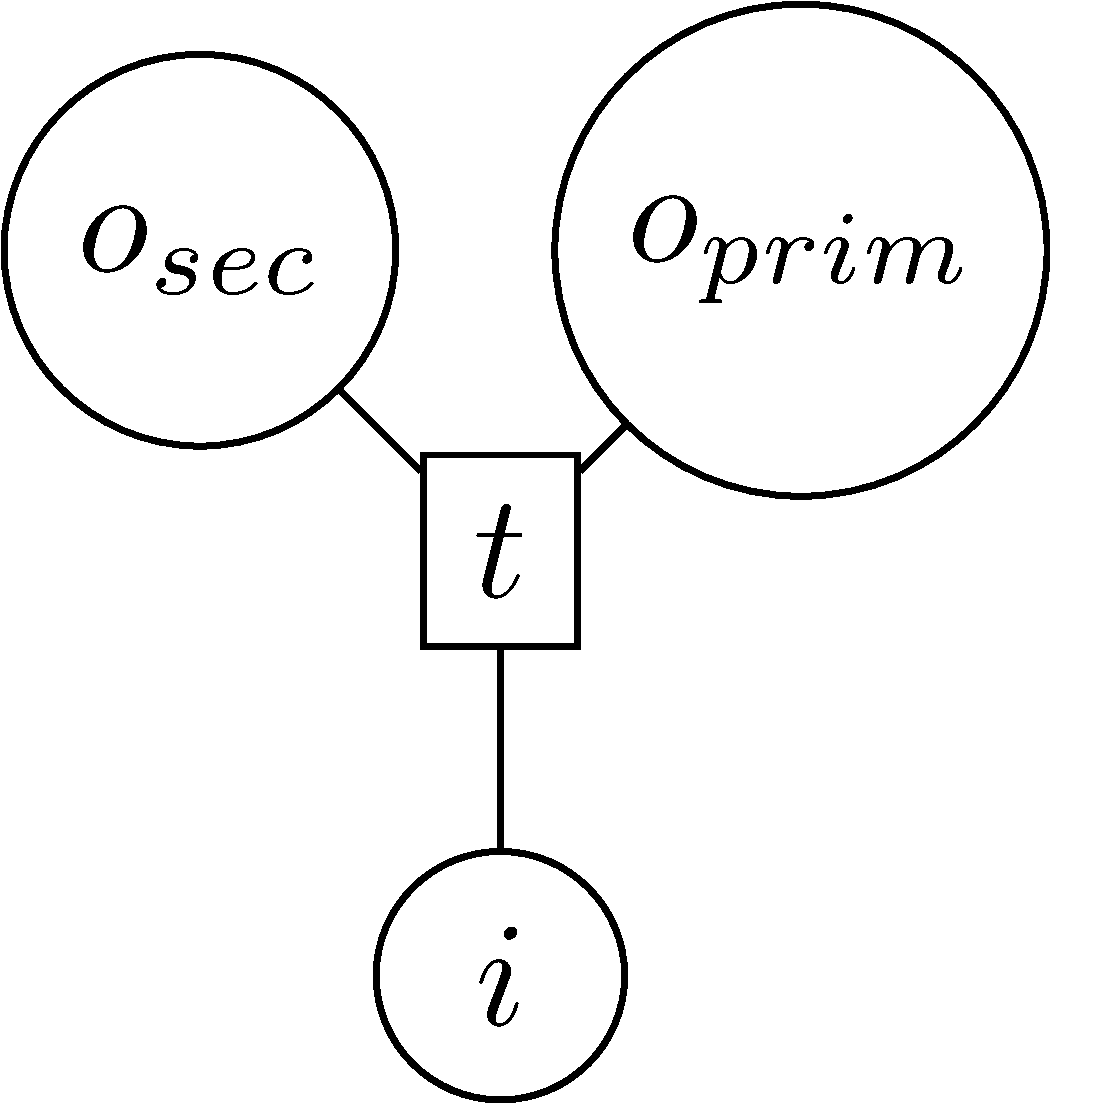
\includegraphics[width=0.5\textwidth]{./imgs/unclust.pdf}
  \caption{\label{fig:org8d8d9a2}The structure of a \texttt{UnClust}.}
\end{figure}


\begin{figure}[p]
  \centering
  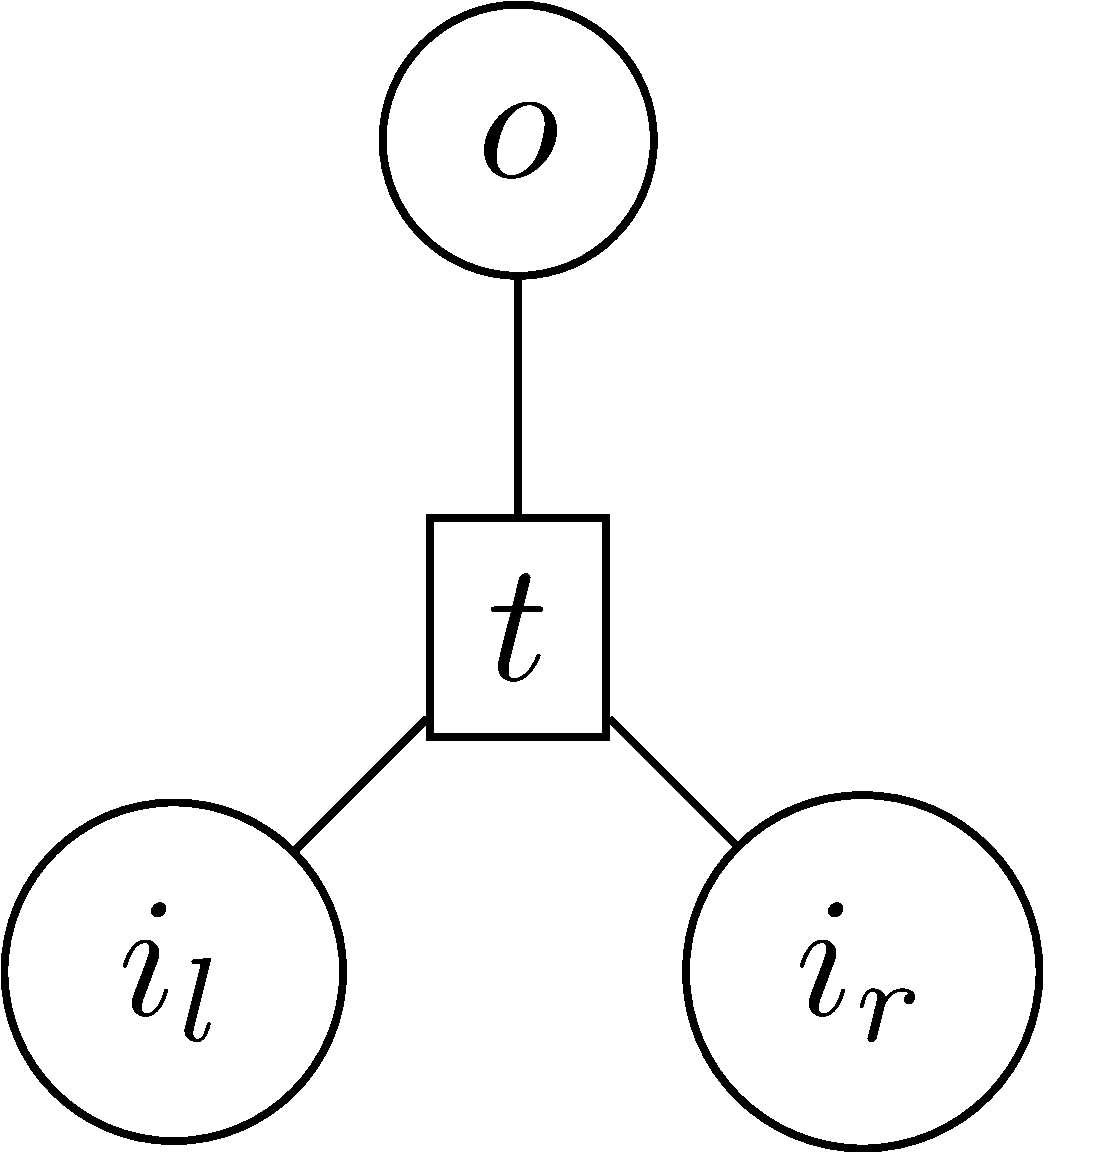
\includegraphics[width=0.5\textwidth]{./imgs/binclust.pdf}
  \caption{\label{fig:org71a57f1}The structure of a \texttt{BinClust}.}
\end{figure}


\begin{figure}[p]
  \centering
  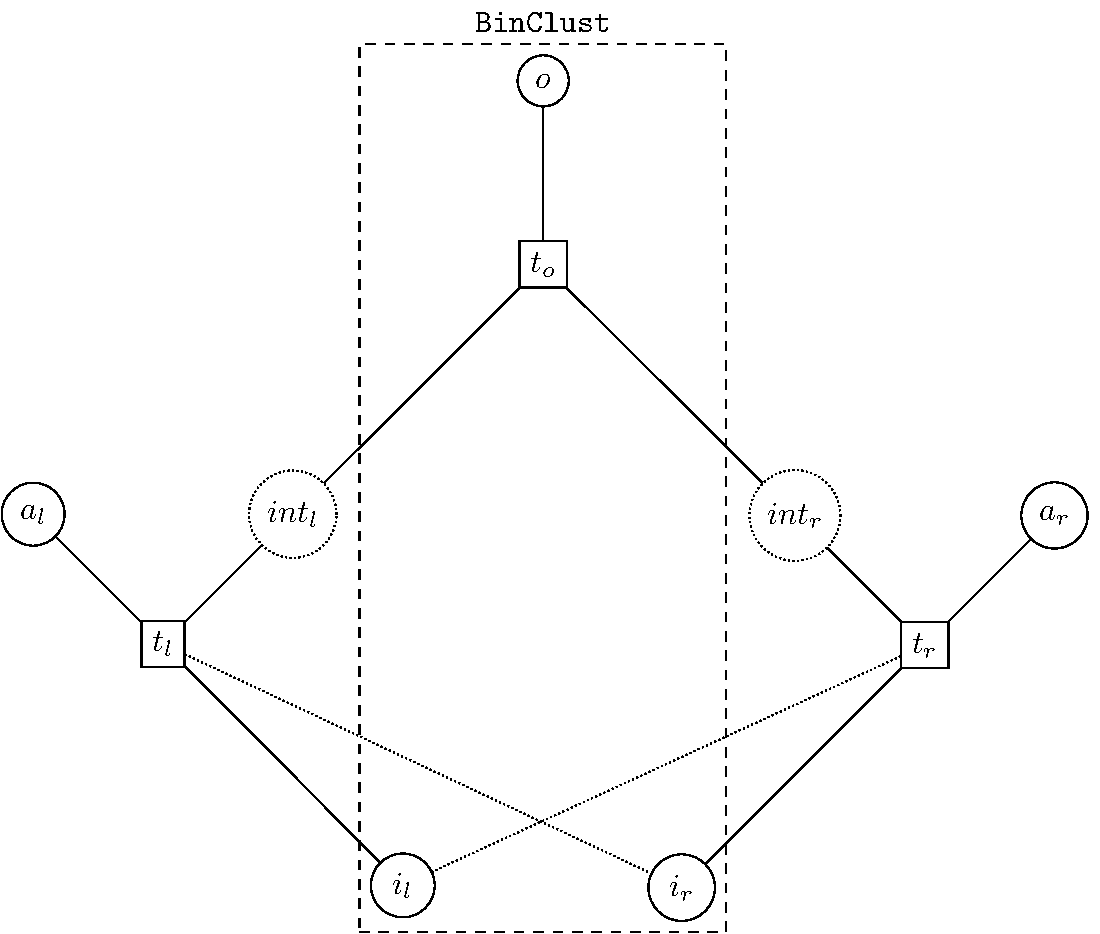
\includegraphics[width=.9\linewidth]{./imgs/joinclust.pdf}
  \caption{\label{fig:orgf1d2858}The structure of a \texttt{JoinClust} notice how it contains a \texttt{BinClust}.}
\end{figure}


\subsection{Populating the graph}
\label{sec:orgf8560ae}
Once the query is transformed into a possible-join forest as described
in the section on \hyperref[sec:org2eb887b]{Possible joins}, the query is transformed into a
forest (listing \ref{org59b4349}) of plans we can insert it into
the tree. This is an iterative process where each operation in each of
the trees in the forest is translated to a cluster which is then
inserted into the DAG. The process if inserting a sub-forest or
sub-tree into the \hyperref[sec:org5a9ec3b]{QDAG} has the effect of extending the QDAG by the
connected clusters corresponding to the operators at the nodes of the
forest, and also returns an n-node that corresponds the sub-forest or
sub-tree relation. However since the insertion function is idempotent,
that is inserting the same forest in the DAG once or twice has no
effect either on the returned value or on the resulting DAG, we
memoize the function. Since the same function recursively inserts all
sub-trees and sub-forests we get for free the mechanism of not
traversing the same tree twice during insertion.

\begin{listing}[p]
  \begin{haskell}
    data QueryForest e s =
    QueryForest
    { qfHash :: Int
      ,qfQueries --
      :: Either --
      (NEL.NonEmpty (Query e (QueryForest e s))) -- An actual forest
      (s,QueryShape e s) -- A final leaf
    }
  \end{haskell}
  \caption{\label{org59b4349}The definition of the query forest. The query forest is hashed so that we can avoid traversing the  same query forest repeatedly. The query forest is essentially a non-empty of queries  with forests at their leafs.}
\end{listing}

The process of traversing the forest and inserting the clusters in the
graph is fairly straightforward. The actual creatin of the clusters,
however, is slightly more convoluted. First a cluster of a type
corresponding to the query operation at the forest node is created
(see section on \hyperref[sec:orgadee761]{cluster polymorphism}). That cluster initially contains
QNF forms at its edges. The QNF forms are then matched against
existing QNFs in the QDAG and the missing ones are generated. If no
new nodes were generated and the matched nodes all correspond to the
same existing cluster, we infer that the cluster is already in the
QDAG and the process finishes . Otherwise we need to create and insert
a clustera and a corresponding \hyperref[sec:org089acdd]{propagator}. Finally all new nodes, QNFs
and the cluster are registered and cross matched so they are easy to
look up. We memoize the entire process using the \texttt{qfHash} to avoid
re-traversing the same path.




\section{Section: query shapes}
\label{sec:org2633f87}
In the section on \hyperref[sec:org9e7f455]{QNFs} we discussed the need to abstract away
infomration that pretains to the particular structure of a query in
favor of semantic information that is rewrite and data
independent. Query shapes cover the opposite need: they encode the
particular cardinality and shape of a relation a specific point in
time.

\subsection{Query Shape}
\label{sec:org17d410b}
A query shape is a datastructure that contains information about the
shape  of a query.

\begin{haskell}
  data QueryShape' e' =
  QueryShape
  { qpSchema :: [(e',ColumnProps)]
    ,qpUnique :: NEL.NonEmpty (NEL.NonEmpty e')
    ,qpSize :: QuerySize
  }
  type QueryShape e s = QueryShape' (ShapeSym e s)
  data ShapeSym e s =
  ShapeSym { planSymQnfName :: QNFName e s
    ,planSymQnfOriginal :: e
  }
  deriving (Show,Generic)
\end{haskell}

A shape contains all combinations that create a uniques subtuple. This
is useful among other places to determine foreign key joins. In a join
like

\begin{minted}[]{sql}
  SELECT * FROM t1,t2 WHERE t1.a = t2.uid
\end{minted}

The resulting table has cardinality at most the size of t1 because
each row of \texttt{t1} matches at most one row of \texttt{t2}. FluiDB does not
support functional dependencies but realistically the column \texttt{a} will
usually be a foreign and therefore the cardinality of the resulting
table will be exactly the cardinality of \texttt{t2}. But what if \texttt{t2} is
actually a subquery things become more complex. Consider the example

\begin{minted}[]{sql}
  SELECT *
  FROM t1,(SELECT * FROM t2,t3)
  WHERE t1.a = t2.uid
\end{minted}

Here \texttt{t2.uid} is part of the unique subtuple but it does not contain
unique values in \texttt{SELECT * FROM t2,t3}. However, the pair \texttt{t2.uid} and
\texttt{t3.uid} together are indeed unique. Therefore we abolish the notion
of unique columns in favour of the notion of uniques subtuples.

This is taken a step furthen when one considers which is the unique
unique in the latter example. One might say \texttt{t1.uid}, \texttt{t2.uid} and
\texttt{t3.uid}. But that is only partially correct as another unique tuple
would be \texttt{t1.uid}, \texttt{t1.a} and \texttt{t3.uid} due to the equality \texttt{t1.a =
  t2.uid}. As stated above FluiDB does not keep track of functional
dependencies, instead it keeps an explicit set of unique subtuples.

To generalize slightly

\begin{itemize}
\item when relations \texttt{A} and \texttt{B} are joined or their product is computed,
  we concatenate all combinations their unique subtuples to come up
  with the new set of unique subtuples.
\item The unique subtuples of a selection are the same as the unique
  subtuples for the underlying relation.
\end{itemize}


\subsection{Shape propagators}
\label{sec:org089acdd}
\hyperref[sec:org17d410b]{Shape} propagators are based on the the idea of the propagator as first
explained in \cite{sussmanArtPropagator2009} and more in depth in
\cite{hansonSoftwareDesignFlexibility2021a}. Very briefly a propagator
network is a hypergraph of cells contianing mutable state and
hyperedges as multi-directional functions that, when triggered, update
the state of the connected cells so they are consistent with each
other. The state of each cell represents some information about a
value (like a bound or a value paired with a certainty metric), and
the propagator takes into account the state of each cell and
propagates that information to the other cells (for example tightening
their bound or finding a linear combination of the alternative values
based on the certainty of each). Kmett \cite{kmettPropagators2021}
formalized the notion of "information about a value" drawing from
\cite{kuperLVarsLatticebasedData2013} encoding it as a lattice with
\(\top\) meaning contradiction, and \(\bot\) meaning that there is no
information about the value. Then the new values of cells are being
joined ( \(\lor\) ) with the old ones and the value is updated to
reflect the combination of information. The example provided by Kmett
is cell being embedded in a 3 level lattice where the bottom level is
\texttt{Nothing}, the middle level is \texttt{Just x} and the top level being a
haskell error.

As the name of our propagator implementation suggests, our idea is to
correspond each cluster to a propagator to form a propagator network
that computes the shapes of the relations corresponding to n-nodes.

Intuitively we model a propagator as a partial function that changes
the values at the edges of a \hyperref[sec:org6e4b098]{cluster}. At construction, each cluster is
equipped with a propagator which, when triggered synchronizes the
values at the edges of the cluster. The partiallity of the function
stems from the fact that it might detect irreconcilable
inconsistencies between the cells (see listing \ref{org945807f}). This
conception of the propagator departs slightly form the conception
described in the paper in that it clearly separates the \emph{cluster} as a
datastructure that holds a fixed number of interdependent values and
the function that updates the values in that cluster.


\begin{listing}[p]
  \begin{haskell}
    type ACPropagator a e s t n =
      EndoE e s (PropCluster a NodeRef e s t n)
    type EndoE e s x = x -> Either (AShowStr e s) x
    type ShapeCluster f e s t n = PropCluster (QueryShape e s) f e s t n
    type PropCluster a f e s t n =
      AnyCluster' (ShapeSym e s) (WMetaD (Defaulting a) f) t n
    newtype WMetaD a f b = WMetaD { unMetaD :: (a,f b)}
      \end{haskell}
  \caption{\label{org945807f}A propagator matches a cluster with shapes at the edges to the same kind of cluster with the shapes synchronized.}
\end{listing}

Given a cluster with n-nodes at the edges we lookup the shape of each
node and add that to the cluster edge. Then the cluster is triggered
Once a cluster is triggered and the values synchoinized those values
are checked against the old ones and for the ones that were updated we
find the clusters in which they participate and run the same
process. The convergence of this process is justified in
\cite{kuperLVarsLatticebasedData2013}.


\subsection{Defaulting functor}
\label{sec:org1d77ea1}
While discussing propagators we mentioned that the cells of a
propagator involve more structure than raw values. Indeed, FluiDB
wraps these values in a functor that we dub as \emph{defaulting functor} to
resason about the consistency of the query shape. In particular we
require that the cell can handle cases where a) the value for the
shape is not computed yet, b) the shape was inferred via the
propagator network and is therefore subject to change and c) the shape
stored in the cell corresponds to a materialized node and other parts
of the FluiDB's internal state are dependent on it. The latter point
is salient. Different logical plans can lead to different, yet
semantically equivalent as per the FluiDB RA.

The defaulting functor (DF) may hold up to two values (see listing
\ref{org4edd50c}).

\begin{itemize}
\item An empty DF means we have no information about the value.
\item a single value (the "default" value) coresponds to a derived shape
  that was computed using the propagator network. The default value is
  updated when propagators are triggered.
\item A full value exists alongside a default value and is constant
  through its lifetime as it matches the value of some state that is
  external to the propagator network, in our particular application it
  represents the shape of a materialized relation. Until that relation
  is delete the registered shape is not allowed to change.
\end{itemize}
\begin{listing}[p]
  \begin{haskell}
    data Defaulting a =
      DefaultingEmpty
      | DefaultingDef a
      | DefaultingFull a a\end{haskell}
  \caption{\label{org4edd50c}The defaulting functor.}
\end{listing}

Since instances of the DF are meant to accomodate propagator values,
adhering to Kmett's approach to cell value maintenance, we define a
semilattice over the DF and define it in terms of a monoid (listing
\ref{orgd554576} ). In partic

Semigroups are not commutative so we give meaning to the order. The
left operand of the semigroup operator is the newer value and the
right one is the older value. Therefore the DF does not require all
the properties of the semilattice which is required to commutative and
associative. In general the semigroup implemented by the underlying
type of the DF is taken to mean \texttt{better <> backup}, i.e. keep as much
of the left oparand as possible unless the right operand is found to
be better for some definition of better. In the case of query shapes
it means keep the schema from the left hand side and the more certain
size.

Bringing our attention to the implementation of the \texttt{Def <> Full}
combination: it inverts the order of combination of the default
values. The reason we do this is to give priority the the full valued
(materialized) nodes when propagating to their immediate neighbors. We
need this when commiting an operator to the code-generation.

\begin{listing}[p]
  \begin{haskell}
    instance Semigroup a => Semigroup (Defaulting a) where
      DefaultingEmpty <> a = a
        a <> DefaultingEmpty = a
      DefaultingDef a <> DefaultingDef a' = DefaultingDef $ a <> a'
      DefaultingDef a <> DefaultingFull a' b' =
        DefaultingFull (a <> a') b'
      DefaultingFull a b <> DefaultingDef a' =
        DefaultingFull (a <> a') b
      DefaultingFull a b <> DefaultingFull a' _ =
        DefaultingFull (a' <> a) b

    instance Semigroup a => Monoid (Defaulting a) where
      mempty = DefaultingEmpty\end{haskell}
  \caption{\label{orgd554576}The join semilattice that is defined in terms of the}
\end{listing}

When commiting to a query plan we are also commiting to full values
for the defaulting values in the propagator cells. Every operator of
the plan corresponds to a query shape propagator. When commiting an
operator to the plan by translating it into C++ code, we promote all
the defaulting values at the edges. It is clear that for the generated
code expects a certain data layout and therefore the \emph{full parts of
  the values must be structurally consistent with each other}. As we
went over in the previous sections, however the default values are
consistent in the amount of information they hold, not in the
structure of the query shape. To facilitate that, before promoting the
default values to full values we trigger the propagator to enforce
full consistency between the values.

The full part and the default part of the the defaulting value are not
necessarily structurally synchronized. We \textbf{internally synchronise} a
cell before triggering the propagator to make sure we maintain the
consistency of the newly promoted cells with the already existing full
cells.

It is notable that there is no formal guarantee that the propagator
will be able to create structurally consistent cells. In that case the
propagator will fail. Handling of this failure is beyond the current
scope of this work.

When an n-node is to be materialized, the corresponding defaultint
functor containing the value is \emph{promoted}.  Promotion of propagators
is copying the default value of a non-full prpagator to the full
state (listing \ref{org20633ba}).


\begin{listing}[p]
  \begin{haskell}
    promoteDefaulting :: Defaulting a -> Defaulting a
    promoteDefaulting = \case
      DefaultingEmpty        -> DefaultingEmpty
      DefaultingDef x        -> DefaultingFull x x
      d@(DefaultingFull _ _) -> d
   \end{haskell}
  \caption{\label{org20633ba}Promoting of defaulting functor happens during code generation when an n-node is materialized.}
\end{listing}

\section{Conclusion}
\label{sec:org75594df}
In this chapter we saw in detail how FluiDB processes queries. From
parsing to generating a graph of queries and inferring the shapes of
the relations in that graph. We also discussed different conceptions
of relational algebra that are used in FluiDB (normal RA and QNF) and
reverse operations. This will serve as a sold bedrock on which we can
build the query planner and on top of that the code generator.

There are a few shortcomings to this model that we have not yet
addressed that we plan to implement in later incarnations of
FluiDB. The most important ones being:

\begin{itemize}
\item As things stand the QDAG will keep growing infinitely as new queries
  arrive and there is no obvious way to prune it while guaraneeing the
  materializability of all the nodes.
\item There is no obvious path to supporting updates in the primary
  tables. There has been a lot of work on materialized view
  maintenance [refs] but most of it assumes that the primary tables
  are also materialized.
\end{itemize}
